% ===========================================================================
% Paper II: Tool Interface Layer — Composition, Capabilities, and the
%           Elixir/OTP Reference Implementation
% Series: The AI Operating System (Part II of V)
% ===========================================================================
\documentclass[12pt,a4paper]{article}

% ---------- packages ----------
\usepackage[utf8]{inputenc}
\usepackage[T1]{fontenc}
\usepackage{lmodern}
\usepackage[margin=1in]{geometry}
\usepackage{amsmath,amssymb,amsthm,mathtools}
\usepackage{tikz}
\usetikzlibrary{arrows.meta,positioning,calc,shapes.geometric,decorations.pathmorphing,fit}
\usepackage[colorlinks=true,linkcolor=blue,citecolor=blue,urlcolor=blue]{hyperref}
\usepackage[round]{natbib}
\usepackage{fancyhdr}
\usepackage{listings}
\usepackage[ruled,vlined,linesnumbered]{algorithm2e}
\usepackage{enumitem}
\usepackage{booktabs}
\usepackage{tabularx}
\usepackage{xcolor}
\usepackage{float}
\usepackage{caption}
\usepackage{everypage}
\usepackage{eso-pic}

% ---------- GrokRxiv sidebar ----------
\definecolor{grokgray}{RGB}{110,110,110}
\AddEverypageHook{%
  \ifnum\value{page}=1
    \begin{tikzpicture}[remember picture, overlay]
      \node[
        rotate=90,
        anchor=south,
        font=\Large\sffamily\bfseries\color{grokgray},
        inner sep=0pt
      ] at ([xshift=38pt, yshift=0.52\paperheight]current page.south west)
      {GrokRxiv:2026.03.tool-interface-ai-os\quad
       [\,cs.AI\,]\quad
       10 Mar 2026};
    \end{tikzpicture}
  \fi
}

% ---------- theorem environments ----------
\theoremstyle{plain}
\newtheorem{theorem}{Theorem}[section]
\newtheorem{lemma}[theorem]{Lemma}
\newtheorem{proposition}[theorem]{Proposition}
\newtheorem{corollary}[theorem]{Corollary}

\theoremstyle{definition}
\newtheorem{definition}[theorem]{Definition}
\newtheorem{example}[theorem]{Example}
\newtheorem{remark}[theorem]{Remark}
\newtheorem{designprinciple}[theorem]{Design Principle}

% ---------- code listings ----------
\definecolor{codebg}{RGB}{248,248,248}
\definecolor{codeframe}{RGB}{200,200,200}
\definecolor{keyword}{RGB}{0,0,180}
\definecolor{comment}{RGB}{0,128,0}
\definecolor{string}{RGB}{163,21,21}
\definecolor{elixirpurple}{RGB}{112,48,160}

\lstdefinelanguage{elixir}{
  keywords={def,defp,defmodule,do,end,fn,use,require,import,alias,case,cond,if,else,
            when,with,for,receive,after,try,catch,rescue,raise,throw,spawn,send,
            defstruct,defprotocol,defimpl,quote,unquote,@,true,false,nil,not,in,
            GenServer,Supervisor,Application,Agent,Task,Process},
  sensitive=true,
  morecomment=[l]{\#},
  morestring=[b]",
  morestring=[b]',
  literate={|>}{{{\color{elixirpurple}|>}}}2
           {->}{{{\color{elixirpurple}->}}}2
           {=>}{{{\color{elixirpurple}=>}}}2
           {<-}{{{\color{elixirpurple}<-}}}2,
}

\lstset{
  backgroundcolor=\color{codebg},
  frame=single,
  rulecolor=\color{codeframe},
  basicstyle=\footnotesize\ttfamily,
  keywordstyle=\color{keyword}\bfseries,
  commentstyle=\color{comment}\itshape,
  stringstyle=\color{string},
  numbers=left,
  numberstyle=\tiny\color{gray},
  numbersep=8pt,
  breaklines=true,
  breakatwhitespace=true,
  tabsize=2,
  showstringspaces=false,
  captionpos=b,
  aboveskip=12pt,
  belowskip=8pt,
}

\lstdefinelanguage{typescript}{
  keywords={import,from,export,default,const,let,var,function,return,if,else,for,while,
            do,switch,case,break,continue,new,this,typeof,instanceof,class,extends,
            implements,interface,type,enum,async,await,try,catch,finally,throw,
            true,false,null,undefined,void,never,any,string,number,boolean,
            as,in,of,readonly,abstract,static,private,public,protected},
  sensitive=true,
  morecomment=[l]{//},
  morecomment=[s]{/*}{*/},
  morestring=[b]",
  morestring=[b]',
  morestring=[b]`,
}

% ---------- page style ----------
\pagestyle{fancy}
\fancyhf{}
\fancyhead[L]{\footnotesize\textit{The AI Operating System, Part II}}
\fancyhead[R]{\footnotesize\textit{Tool Interface Layer}}
\fancyfoot[C]{\thepage}
\renewcommand{\headrulewidth}{0.4pt}

% ---------- custom commands ----------
\newcommand{\agenthero}{\textsc{Agent-Hero}}
\newcommand{\MCP}{\textsc{mcp}}
\newcommand{\pipe}{\;|\!\!>\;}

% ===========================================================================
\begin{document}

% ---------- title ----------
\begin{center}
  {\LARGE\bfseries The AI Operating System, Part II:\\[4pt]
  Tool Interface Layer --- Composition, Capabilities,\\[2pt]
  and the Elixir/OTP Reference Implementation}

  \bigskip

  {\large Matthew Long}\\[4pt]
  The YonedaAI Collaboration\\
  YonedaAI Research Collective\\
  Chicago, IL\\[2pt]
  \texttt{matthew@yonedaai.com} \textperiodcentered{} \texttt{https://yonedaai.com}

  \bigskip

  {\small March 10, 2026}
\end{center}

\bigskip

% ===== ABSTRACT =====
\begin{abstract}
\noindent
An AI Operating System mediates every interaction between intelligent agents and the external world through a \emph{tool interface layer} that is analogous to the device-driver subsystem of a classical operating system. In this second paper of a five-part series, we design a tool interface layer built on the principles of functional composition, capability-based security, and sandboxed execution. The design centres on a three-tier tool registry---Builtin, Sandbox, and MCP (Model Context Protocol)---where tools are higher-order functions composed through pipelines, access is governed by HMAC-signed capability tokens with time-to-live and rate limiting, and untrusted code executes in isolated BEAM processes with hard timeouts. We present a complete reference implementation in Elixir/OTP comprising six modules: a GenServer-based registry with freeze semantics, a cryptographic capability token system, a process-isolated sandbox executor, a JSON-RPC MCP protocol client with parallel discovery, an asynchronous audit logger with telemetry integration, and a facade module that composes these components into a single invocation pipeline. The implementation exploits the BEAM virtual machine's natural properties---per-process heap isolation, preemptive scheduling, supervision trees, and message-passing concurrency---to achieve the security and reliability guarantees that classical operating systems obtain through hardware-enforced protection rings. We validate the design against the \agenthero{} production platform, where the three-tier model maps directly to builtin tools, E2B ephemeral sandboxes, and \texttt{StreamableHTTPClientTransport}-based MCP connections. Comparisons are drawn to Unix device drivers, Plan~9, Capsicum capabilities, and seL4 verified security.

\medskip
\noindent\textbf{Keywords:} AI operating system, tool interface, capability-based security, Model Context Protocol, functional composition, Elixir/OTP, sandboxing, pipeline operators, higher-order functions
\end{abstract}

\tableofcontents
\newpage

% ===== 1. INTRODUCTION =====
\section{Introduction}
\label{sec:intro}

The fundamental architectural insight of classical operating systems is that application code must never interact with hardware directly. Instead, a layer of \emph{device drivers} interposes between user-space programs and peripheral devices, providing abstraction, multiplexing, isolation, and auditability~\citep{tanenbaum2014modern}. An application opens a file descriptor, reads and writes through a well-defined system-call interface, and the kernel routes those operations to the appropriate driver. The application need not know whether the underlying device is a local disk, a network socket, or a USB peripheral.

In an AI Operating System, the same architectural principle applies with even greater force. Agents---large language models with autonomy over their computational environment---must interact with external systems: databases, web APIs, file systems, code interpreters, and other agents. These interactions are mediated by \emph{tools}: typed functions that accept structured input and return structured output, with well-defined security boundaries, execution constraints, and audit trails.

This paper develops the design and implementation of the tool interface layer. Our approach is rooted in functional programming: tools are composable functions, security is enforced through unforgeable capability tokens, isolation is achieved through process boundaries, and the entire invocation pipeline is a composition of pure validation, authorized execution, and audit logging. While the underlying ideas can be formalized using category theory (tools as morphisms, capabilities as representable functors), we focus on the engineering design and its concrete realization in Elixir/OTP.

\paragraph{Contributions.} Our contributions are:

\begin{enumerate}[leftmargin=2em]
\item A \textbf{three-tier tool registry design} (Builtin, Sandbox, MCP) with freeze semantics that locks tool configurations at execution time, preventing privilege escalation through dynamic discovery (Section~\ref{sec:design}).

\item A \textbf{capability-based security model} using HMAC-signed tokens with time-to-live, rate limiting, and permission scoping, enforcing the Principle of Least Authority without centralized access control lists (Section~\ref{sec:capabilities}).

\item A \textbf{sandboxed execution model} using BEAM process isolation with monitored timeouts, providing the same isolation guarantees as E2B ephemeral environments but at the language-runtime level (Section~\ref{sec:sandbox}).

\item A \textbf{complete Elixir/OTP reference implementation} comprising six modules totaling approximately 700 lines, with GenServer state machines, supervision trees, and telemetry integration (Sections~\ref{sec:facade}--\ref{sec:audit}).

\item A \textbf{MCP protocol client} with session management, parallel multi-server discovery via \texttt{Task.async\_stream}, and closure-based remote execution (Section~\ref{sec:mcp}).

\item \textbf{Production validation} against the \agenthero{} platform, demonstrating that the reference implementation's design maps directly to a deployed system handling real agent workloads (Section~\ref{sec:production}).
\end{enumerate}

\paragraph{Relation to the series.} This is Part~II of a five-part series on the AI Operating System. Part~I~\citep{longyoneda2026kernel} established the kernel architecture---the process model and scheduling layer. The present paper builds on that foundation by defining the interface through which scheduled agent processes access external capabilities. Part~III will address memory and persistence, Part~IV the agent orchestration layer, and Part~V the integration of all components.

\paragraph{Notation.} We use Elixir syntax throughout. The pipe operator \texttt{|>} denotes left-to-right function composition: \texttt{x |> f |> g} means ``apply \texttt{f} to \texttt{x}, then apply \texttt{g} to the result.'' Pattern matching on tagged tuples (\texttt{\{:ok, value\}} and \texttt{\{:error, reason\}}) provides exhaustive error handling. The \texttt{with} expression chains multiple pattern-matched operations, short-circuiting on the first failure.


% ===== 2. BACKGROUND =====
\section{Background and Motivation}
\label{sec:background}

\subsection{Device Drivers and the Abstraction Principle}

The device driver model in Unix-like operating systems provides three critical properties~\citep{love2010linux}:

\begin{enumerate}[leftmargin=2em]
\item \textbf{Abstraction.} Applications interact with a uniform file-descriptor interface regardless of the underlying device.
\item \textbf{Isolation.} A misbehaving driver cannot corrupt unrelated kernel state, especially in microkernel designs.
\item \textbf{Multiplexing.} Multiple processes can share a single device through the driver's queuing and scheduling logic.
\end{enumerate}

Plan~9 from Bell Labs extended this model to its logical conclusion: every resource---networks, graphics, even per-process name spaces---is presented as a file system~\citep{pike1995plan9}. This ``everything is a file'' philosophy provides a universal interface that any program can consume without special-purpose client libraries. The AI OS tool layer aspires to the same universality: every external capability, whether a web search engine, a code interpreter, or a third-party API, is accessed through the same typed invocation protocol.

\subsection{Capability-Based Security}

Traditional access control uses access control lists (ACLs) attached to resources. Capability-based security inverts this: each subject holds unforgeable \emph{capability tokens} that grant specific permissions on specific objects~\citep{dennis1966capabilities,levy1984capability}. Modern realizations include:

\begin{itemize}[leftmargin=2em]
\item \textbf{Capsicum} (FreeBSD): capability mode restricts a sandboxed process to only the file descriptors it was given at entry~\citep{watson2010capsicum}.
\item \textbf{seL4}: a formally verified microkernel where every system call requires a capability argument~\citep{klein2009sel4}.
\item \textbf{WASI} (WebAssembly System Interface): capability-based access to host resources from sandboxed WebAssembly modules~\citep{wasi2023spec}.
\item \textbf{Macaroons}: decentralized capability tokens with contextual caveats for distributed systems~\citep{birgisson2014macaroons}.
\end{itemize}

The AI OS adapts capability-based security to the agent setting: each agent holds a set of capability tokens that determine which tools it may invoke, with what parameters, and at what rate. Tokens are cryptographically signed, time-bounded, and rate-limited---unforgeable values that travel with the agent rather than being stored in a central authority.

\subsection{The BEAM Virtual Machine}

The BEAM virtual machine (Erlang/Elixir runtime) provides properties that make it an ideal substrate for a tool interface layer~\citep{armstrong2003erlang,juric2019elixir}:

\begin{itemize}[leftmargin=2em]
\item \textbf{Process isolation}: Each process has its own heap. There is no shared mutable state between processes.
\item \textbf{Message passing}: Processes communicate only through asynchronous, copied messages.
\item \textbf{Preemptive scheduling}: The BEAM scheduler preempts processes after a reduction count, preventing any single tool execution from starving others.
\item \textbf{Supervision trees}: Processes are organized hierarchically; a supervisor restarts failed children according to a declared strategy.
\item \textbf{Hot code loading}: Modules can be upgraded at runtime without stopping the system.
\end{itemize}

These properties mean that BEAM process isolation provides the same security boundary that classical operating systems achieve through hardware protection rings. A sandboxed tool execution in a spawned BEAM process cannot read the parent's memory, cannot access file descriptors it was not given, and is automatically cleaned up if it crashes or times out.

\subsection{Functional Programming as Design Language}

We frame the tool interface layer using the vocabulary of functional programming rather than, say, object-oriented design patterns or formal category theory. The key concepts are:

\begin{itemize}[leftmargin=2em]
\item \textbf{Composition}: Tools are functions that compose. The output of one tool feeds into the input of the next. Composition is associative: \texttt{x |> f |> g |> h} produces the same result regardless of how we parenthesize the intermediate steps.
\item \textbf{Higher-order functions}: Tools are values. A tool's \texttt{execute} field holds a function (\texttt{fn input -> \{:ok, result\} end}). This function can be stored, passed, composed, and wrapped.
\item \textbf{Closures}: The MCP client constructs remote execution functions as closures that capture the server URL, authentication token, and session ID. The caller invokes the closure without knowing it dispatches over HTTP.
\item \textbf{Pattern matching}: Authorization, validation, and dispatch are implemented as pattern matches on tagged tuples, providing exhaustive case analysis and clear error paths.
\item \textbf{Pipeline operators}: The invocation pipeline---authorize, validate, execute, audit---is a left-to-right composition expressed with \texttt{with} and \texttt{|>}.
\end{itemize}

\begin{remark}[Categorical background]
For readers familiar with category theory, the design has a clean categorical interpretation: tools are morphisms in a typed category, capability tokens correspond to the representable functor $\mathrm{Hom}(T, -)$, and sandboxing is a passage to a restricted subcategory. The Yoneda lemma guarantees that capability tokens faithfully represent tools. We do not develop this formalism here, but note that the functional programming concepts above are the computational counterparts of these categorical structures.
\end{remark}


% ===== 3. THREE-TIER TOOL REGISTRY =====
\section{Three-Tier Tool Registry Design}
\label{sec:design}

\subsection{Design Overview}

The tool interface layer organizes tools into three tiers based on trust level and execution model. Each tier represents a different trade-off between flexibility and security:

\begin{designprinciple}[Tiered Trust]
\label{dp:tiers}
Tools are partitioned into three tiers with decreasing trust and increasing isolation requirements:
\begin{enumerate}
\item \textbf{Builtin} --- Statically defined, trusted operations that execute in the registry process itself.
\item \textbf{Sandbox} --- Operations requiring isolated execution in a separate BEAM process with hard timeouts.
\item \textbf{MCP} --- Runtime-discovered tools from external Model Context Protocol servers, accessed over HTTP.
\end{enumerate}
\end{designprinciple}

The three tiers are not an arbitrary partition. They correspond to three fundamentally different trust relationships:

\begin{itemize}[leftmargin=2em]
\item \textbf{Builtin tools} are authored by the platform developers, reviewed, tested, and deployed as part of the system. They run in the same trust domain as the registry. Examples: \texttt{web-search}, \texttt{text-transform}, \texttt{web-scrape}, \texttt{pdf-parse}, \texttt{generate-document}, \texttt{spreadsheet-read}.

\item \textbf{Sandbox tools} execute code that may come from untrusted sources (agent-generated code, third-party scripts). They must be isolated: separate heap, hard timeout, monitored lifecycle. Examples: \texttt{git-clone}, \texttt{npm-run}, \texttt{code-exec}, \texttt{file-ops}, \texttt{python-exec}, \texttt{shell-exec}.

\item \textbf{MCP tools} are discovered at runtime from external servers. The platform has no control over their implementation. They are accessed via HTTP with Bearer token authentication and namespaced to prevent collisions: \texttt{\$\{serverName\}\_\_\$\{toolName\}}.
\end{itemize}

\begin{figure}[ht]
\centering
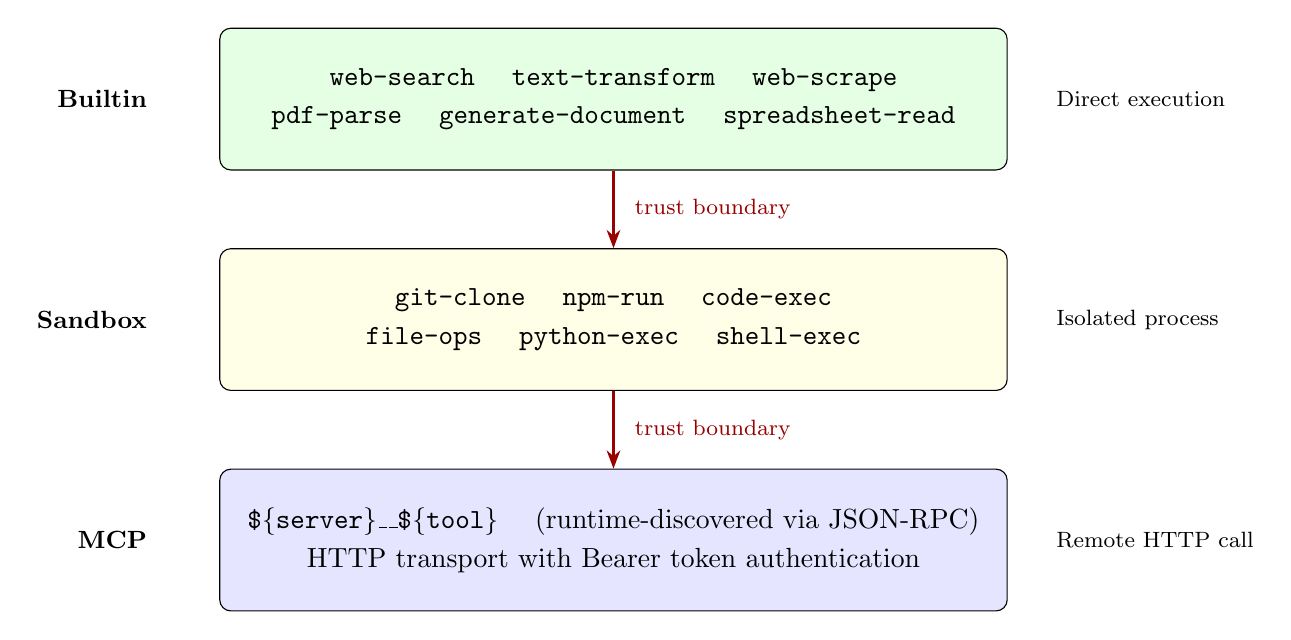
\begin{tikzpicture}[
  tier/.style={draw, rounded corners, minimum width=10cm, minimum height=1.8cm, align=center},
  label/.style={font=\small\bfseries, anchor=east}
]
\node[tier, fill=green!10] (builtin) at (0,0) {
  \texttt{web-search} \quad \texttt{text-transform} \quad \texttt{web-scrape}\\[2pt]
  \texttt{pdf-parse} \quad \texttt{generate-document} \quad \texttt{spreadsheet-read}
};
\node[tier, fill=yellow!10] (sandbox) at (0,-2.8) {
  \texttt{git-clone} \quad \texttt{npm-run} \quad \texttt{code-exec}\\[2pt]
  \texttt{file-ops} \quad \texttt{python-exec} \quad \texttt{shell-exec}
};
\node[tier, fill=blue!10] (mcp) at (0,-5.6) {
  \texttt{\$\{server\}\_\_\$\{tool\}} \quad (runtime-discovered via JSON-RPC)\\[2pt]
  HTTP transport with Bearer token authentication
};
\node[label] at (-5.8,0) {\small Builtin};
\node[label] at (-5.8,-2.8) {\small Sandbox};
\node[label] at (-5.8,-5.6) {\small MCP};

\draw[-{Stealth}, thick, red!60!black] (builtin.south) -- (sandbox.north) node[midway, right=4pt, font=\footnotesize\color{red!60!black}] {trust boundary};
\draw[-{Stealth}, thick, red!60!black] (sandbox.south) -- (mcp.north) node[midway, right=4pt, font=\footnotesize\color{red!60!black}] {trust boundary};

\node[anchor=west, font=\footnotesize] at (5.5, 0) {Direct execution};
\node[anchor=west, font=\footnotesize] at (5.5, -2.8) {Isolated process};
\node[anchor=west, font=\footnotesize] at (5.5, -5.6) {Remote HTTP call};
\end{tikzpicture}
\caption{Three-tier tool registry. Trust decreases from top to bottom; isolation increases correspondingly. Each tier boundary represents a different execution model.}
\label{fig:three-tier}
\end{figure}

\subsection{Tool Specification as a Record Type}

Every tool, regardless of tier, conforms to a common specification. In Elixir, this is expressed as a typed struct:

\begin{lstlisting}[language=elixir, caption={Tool specification type.}, label={lst:tool-spec}]
@type tool_tier :: :builtin | :sandbox | :mcp

@type tool_spec :: %{
  name: String.t(),
  tier: tool_tier(),
  description: String.t(),
  input_schema: map(),            # JSON Schema for input validation
  output_schema: map() | nil,     # JSON Schema for output (optional)
  validate: (map() -> :ok | {:error, term()}) | nil,
  execute: (map() -> {:ok, any()} | {:error, term()})
}
\end{lstlisting}

The critical field is \texttt{execute}: a higher-order function that takes a map of input parameters and returns a tagged result tuple. This is the tool's runtime behavior, captured as a first-class value. For builtin tools, the function runs directly. For sandbox tools, it runs inside an isolated process. For MCP tools, it is a closure that dispatches a JSON-RPC call over HTTP.

The \texttt{validate} field is an optional higher-order function for input validation. When present, it is called before execution. When absent (nil), all inputs are accepted. This allows tools to define custom validation logic beyond what JSON Schema can express---for example, URL safety checks that block localhost and private IP ranges.

\subsection{The Registry GenServer}

The registry is implemented as a \texttt{GenServer}---an OTP behavior that provides a single-threaded, message-driven state machine. The state holds three maps (one per tier) plus a boolean frozen flag:

\begin{lstlisting}[language=elixir, caption={Registry state and initialization.}, label={lst:registry-state}]
defmodule ToolInterface.Registry do
  use GenServer
  require Logger

  defstruct builtin: %{}, sandbox: %{}, mcp: %{}, frozen: false

  def start_link(opts \\ []) do
    GenServer.start_link(__MODULE__, opts, name: __MODULE__)
  end

  @impl true
  def init(_opts) do
    state = %__MODULE__{
      builtin: load_builtin_tools(),
      sandbox: load_sandbox_tools(),
      mcp: %{},
      frozen: false
    }
    Logger.info(
      "[Registry] Initialized with #{map_size(state.builtin)} builtin, " <>
      "#{map_size(state.sandbox)} sandbox tools"
    )
    {:ok, state}
  end
end
\end{lstlisting}

Builtin and sandbox tools are loaded at startup from static definitions. MCP tools start empty and are populated through runtime discovery. The GenServer's single-threaded message processing guarantees that all registry operations---lookup, registration, freezing---are serialized, eliminating race conditions without explicit locks.

\subsection{Lookup: Searching Across Tiers}

Tool lookup searches across all three tiers in priority order (builtin first, then sandbox, then MCP):

\begin{lstlisting}[language=elixir, caption={Tool lookup across tiers.}, label={lst:lookup}]
def handle_call({:lookup, tool_id}, _from, state) do
  result =
    case Map.get(state.builtin, tool_id) ||
         Map.get(state.sandbox, tool_id) ||
         Map.get(state.mcp, tool_id) do
      nil  -> {:error, :not_found}
      tool -> {:ok, tool}
    end
  {:reply, result, state}
end
\end{lstlisting}

The \texttt{||} chain is a pattern common in Elixir: it evaluates left-to-right and returns the first non-nil value. This gives builtin tools priority over sandbox tools, and sandbox tools priority over MCP tools. A builtin \texttt{web-search} cannot be shadowed by an MCP tool with the same name.

\subsection{MCP Registration with Namespacing}

When an MCP server is discovered, its tools are registered with a namespace prefix to prevent collisions:

\begin{lstlisting}[language=elixir, caption={MCP tool registration with namespace and freeze guard.}, label={lst:register-mcp}]
def handle_call({:register_mcp, _server_name, _tools}, _from,
                %{frozen: true} = state) do
  {:reply, {:error, :frozen}, state}
end

def handle_call({:register_mcp, server_name, tools}, _from, state) do
  namespaced =
    for tool <- tools, into: %{} do
      namespaced_name = "#{server_name}__#{tool.name}"
      spec = %{
        name: namespaced_name,
        tier: :mcp,
        description: Map.get(tool, :description, ""),
        input_schema: Map.get(tool, :input_schema, %{}),
        output_schema: Map.get(tool, :output_schema, nil),
        validate: build_mcp_validator(tool),
        execute: Map.get(tool, :execute,
                         fn _ -> {:error, :not_implemented} end)
      }
      {namespaced_name, spec}
    end

  Logger.info("[Registry] Registered #{map_size(namespaced)} " <>
              "MCP tools from #{server_name}")
  {:reply, :ok, %{state | mcp: Map.merge(state.mcp, namespaced)}}
end
\end{lstlisting}

Note the two clauses of \texttt{handle\_call}: the first pattern matches on \texttt{\%\{frozen: true\}} and rejects the registration. The second clause handles the normal case. This is Elixir's pattern matching applied to state machine design---the frozen guard is not a runtime conditional but a structural match on the state.

\subsection{Freeze Semantics: Contract-Locked Configuration}

The freeze operation is the registry's most important security feature:

\begin{lstlisting}[language=elixir, caption={Registry freeze operation.}, label={lst:freeze}]
def handle_call(:freeze, _from, state) do
  total = map_size(state.builtin) +
          map_size(state.sandbox) +
          map_size(state.mcp)
  Logger.info("[Registry] Frozen with #{total} total tools")
  {:reply, :ok, %{state | frozen: true}}
end
\end{lstlisting}

Once frozen, the registry is immutable: no new tools can be registered. This implements the \emph{contract-locked configuration} pattern. When an agent execution begins, the tool set is frozen. The agent cannot discover additional tools or escalate its privileges by connecting to new MCP servers during execution. This is analogous to Capsicum's capability mode~\citep{watson2010capsicum}: once a process enters capability mode, it can only use the file descriptors it already holds.

\begin{designprinciple}[Contract Locking]
\label{dp:freeze}
The set of available tools must be frozen before agent execution begins. No tool registration, deregistration, or modification is permitted during execution. This prevents:
\begin{enumerate}
\item Privilege escalation through dynamic tool discovery.
\item Time-of-check/time-of-use (TOCTOU) vulnerabilities in capability validation.
\item Non-deterministic behavior from changing tool sets mid-execution.
\end{enumerate}
\end{designprinciple}

\subsection{Builtin Tool Definitions}

Builtin tools are defined as maps with higher-order functions for validation and execution. Here is the \texttt{web-search} tool with its input validator:

\begin{lstlisting}[language=elixir, caption={Builtin tool definition with validation function.}, label={lst:builtin-tool}]
%{
  name: "web-search",
  tier: :builtin,
  description: "Search the web using a query string",
  input_schema: %{
    "type" => "object",
    "properties" => %{
      "query" => %{"type" => "string"},
      "max_results" => %{
        "type" => "integer", "minimum" => 1, "maximum" => 20
      }
    },
    "required" => ["query"]
  },
  output_schema: %{
    "type" => "array",
    "items" => %{"type" => "object"}
  },
  validate: &validate_web_search/1,
  execute: fn input ->
    {:ok, %{results: [], query: input["query"]}}
  end
}
\end{lstlisting}

The \texttt{validate} field uses a function capture (\texttt{\&validate\_web\_search/1}) that points to a private function performing domain-specific validation:

\begin{lstlisting}[language=elixir, caption={Pattern-matched input validation.}, label={lst:validate}]
defp validate_web_search(%{"query" => q})
  when is_binary(q) and byte_size(q) > 0, do: :ok
defp validate_web_search(_), do: {:error, :invalid_query}
\end{lstlisting}

This is pure pattern matching: the function has two clauses. The first matches a map with a non-empty binary \texttt{"query"} key and returns \texttt{:ok}. The second is a catch-all that returns an error. There is no conditional logic, no null checking, no exception throwing---just exhaustive pattern matching on the input structure.

\subsection{URL Safety Validation}

Tools that access URLs (\texttt{web-scrape}, \texttt{pdf-parse}, \texttt{git-clone}) share a URL safety validator that blocks access to localhost, loopback, link-local, and private network ranges:

\begin{lstlisting}[language=elixir, caption={URL safety validation blocking internal addresses.}, label={lst:url-safety}]
defp validate_url_string(url) do
  uri = URI.parse(url)
  blocked_hosts = ["localhost", "127.0.0.1", "0.0.0.0", "::1"]
  blocked_prefixes = [
    "169.254.", "10.", "192.168.",
    "172.16.", "172.17.", "172.18.", "172.19.",
    "172.20.", "172.21.", "172.22.", "172.23.",
    "172.24.", "172.25.", "172.26.", "172.27.",
    "172.28.", "172.29.", "172.30.", "172.31."
  ]
  host = uri.host || ""

  cond do
    host in blocked_hosts ->
      {:error, {:blocked_host, host}}
    Enum.any?(blocked_prefixes,
              &String.starts_with?(host, &1)) ->
      {:error, {:blocked_ip_range, host}}
    true ->
      :ok
  end
end
\end{lstlisting}

This prevents Server-Side Request Forgery (SSRF) attacks where an agent tricks a tool into accessing internal infrastructure. The blocked ranges cover the full RFC~1918 private address space plus the AWS metadata endpoint range (\texttt{169.254.x.x}).

\subsection{Listing and Filtering}

The registry supports listing tools filtered by tier, implemented through pattern-matched \texttt{handle\_call} clauses:

\begin{lstlisting}[language=elixir, caption={Filtered tool listing.}, label={lst:list}]
def handle_call({:list, nil}, _from, state) do
  all = Map.values(state.builtin) ++
        Map.values(state.sandbox) ++
        Map.values(state.mcp)
  {:reply, all, state}
end

def handle_call({:list, :builtin}, _from, state) do
  {:reply, Map.values(state.builtin), state}
end

def handle_call({:list, :sandbox}, _from, state) do
  {:reply, Map.values(state.sandbox), state}
end

def handle_call({:list, :mcp}, _from, state) do
  {:reply, Map.values(state.mcp), state}
end
\end{lstlisting}

Each tier filter is its own function clause. Adding a new tier would mean adding a new clause---no modification to existing code. This is the open/closed principle realized through pattern matching.


% ===== 4. CAPABILITY-BASED SECURITY =====
\section{Capability Token System}
\label{sec:capabilities}

\subsection{Design Philosophy}

The tool interface layer uses capability-based access control rather than access control lists. Each agent holds unforgeable tokens that grant specific permissions on specific tools. A token is a value: it can be passed, stored, and validated, but it cannot be forged because it carries a cryptographic signature.

\begin{designprinciple}[Capability Tokens as Values]
\label{dp:cap-values}
Capability tokens are immutable value types, not references to centralized state. A token encodes:
\begin{enumerate}
\item \emph{Who}: the agent identity (\texttt{agent\_id}).
\item \emph{What}: the tool identity (\texttt{tool\_id}).
\item \emph{How}: the permitted operations (\texttt{permissions}).
\item \emph{How fast}: the maximum invocation rate (\texttt{rate\_limit}).
\item \emph{Until when}: the expiry time (\texttt{expires\_at}).
\item \emph{Proof}: the HMAC-SHA256 signature (\texttt{signature}).
\end{enumerate}
\end{designprinciple}

This design has several advantages over centralized ACLs:

\begin{itemize}[leftmargin=2em]
\item \textbf{No central bottleneck}: Authorization is validated locally by checking the token's signature. There is no database lookup, no network call, no single point of failure.
\item \textbf{Offline validation}: A token can be validated without contacting any authority---the HMAC signature is self-contained.
\item \textbf{Fine-grained scoping}: Each token is scoped to exactly one tool. An agent with access to ten tools holds ten tokens.
\item \textbf{Time-bounded}: Tokens expire automatically. Compromised tokens have a limited window of exploitability.
\item \textbf{Rate-limited}: Each token enforces a per-minute invocation cap, preventing abuse even with valid credentials.
\end{itemize}

\subsection{Token Structure}

The capability token is implemented as an Elixir struct with enforced keys:

\begin{lstlisting}[language=elixir, caption={Capability token struct definition.}, label={lst:cap-struct}]
defmodule ToolInterface.Capability do
  @type permission :: :invoke | :inspect | :compose

  @type t :: %__MODULE__{
    agent_id: String.t(),
    tool_id: String.t(),
    permissions: [permission()],
    rate_limit: pos_integer(),
    expires_at: DateTime.t(),
    signature: binary(),
    invocation_count: non_neg_integer(),
    last_reset_at: DateTime.t()
  }

  @enforce_keys [:agent_id, :tool_id, :permissions,
                 :rate_limit, :expires_at, :signature]
  defstruct [
    :agent_id, :tool_id, :permissions,
    :rate_limit, :expires_at, :signature,
    invocation_count: 0,
    last_reset_at: nil
  ]
end
\end{lstlisting}

Three permission levels are defined:

\begin{itemize}[leftmargin=2em]
\item \textbf{\texttt{:invoke}} --- Permission to execute the tool. This is the most common permission.
\item \textbf{\texttt{:inspect}} --- Permission to read the tool's schema and description without executing it.
\item \textbf{\texttt{:compose}} --- Permission to use the tool as part of a composed pipeline with other tools.
\end{itemize}

The \texttt{invocation\_count} and \texttt{last\_reset\_at} fields track rate limiting state. The rate window resets every 60 seconds.

\subsection{Token Creation with HMAC Signing}

Token creation validates parameters and computes an HMAC-SHA256 signature over the token's identity fields:

\begin{lstlisting}[language=elixir, caption={Token creation with cryptographic signing.}, label={lst:cap-create}]
@signing_key "tool_interface_capability_signing_key_v1"

def create(agent_id, tool_id, permissions, rate_limit, ttl_seconds)
    when is_binary(agent_id) and is_binary(tool_id)
    and is_list(permissions)
    and is_integer(rate_limit) and rate_limit > 0
    and is_integer(ttl_seconds) and ttl_seconds > 0 do

  valid_permissions = [:invoke, :inspect, :compose]

  if Enum.all?(permissions, &(&1 in valid_permissions)) do
    expires_at = DateTime.add(DateTime.utc_now(),
                              ttl_seconds, :second)
    token = %__MODULE__{
      agent_id: agent_id,
      tool_id: tool_id,
      permissions: permissions,
      rate_limit: rate_limit,
      expires_at: expires_at,
      signature: <<>>,
      invocation_count: 0,
      last_reset_at: DateTime.utc_now()
    }
    signature = compute_signature(token)
    {:ok, %{token | signature: signature}}
  else
    {:error, :invalid_permissions}
  end
end

def create(_, _, _, _, _), do: {:error, :invalid_parameters}
\end{lstlisting}

The guard clause (\texttt{when is\_binary(agent\_id) and ...}) ensures that the function only matches when all parameters have the correct types. If any parameter is wrong---a nil agent ID, a negative rate limit, a non-integer TTL---the second clause matches and returns \texttt{\{:error, :invalid\_parameters\}}.

The HMAC signature is computed over a canonical string representation of the token's identity fields:

\begin{lstlisting}[language=elixir, caption={HMAC-SHA256 signature computation.}, label={lst:hmac}]
defp compute_signature(%__MODULE__{} = token) do
  payload =
    "#{token.agent_id}:#{token.tool_id}:" <>
    "#{inspect(token.permissions)}:" <>
    "#{token.rate_limit}:" <>
    "#{DateTime.to_iso8601(token.expires_at)}"

  :crypto.mac(:hmac, :sha256, @signing_key, payload)
end
\end{lstlisting}

The signing key would come from a secrets manager in production. The signature binds the token's fields together: modifying any field (agent ID, tool ID, permissions, rate limit, or expiry) invalidates the signature.

\subsection{Authorization: The Five-Check Pipeline}

Token authorization is a pipeline of five checks, implemented as a \texttt{cond} expression:

\begin{lstlisting}[language=elixir, caption={Five-check authorization pipeline.}, label={lst:authorize}]
def authorize(%__MODULE__{} = token, tool_id) do
  cond do
    token.tool_id != tool_id ->
      {:error, :unauthorized}

    :invoke not in token.permissions ->
      {:error, :unauthorized}

    expired?(token) ->
      {:error, :expired}

    not valid_signature?(token) ->
      {:error, :invalid_signature}

    rate_limited?(token) ->
      {:error, :rate_limited}

    true ->
      updated = increment_invocation(token)
      {:ok, updated}
  end
end

def authorize(_, _), do: {:error, :unauthorized}
\end{lstlisting}

The five checks, in order:

\begin{enumerate}[leftmargin=2em]
\item \textbf{Tool match}: The token's \texttt{tool\_id} must match the requested tool. A token for \texttt{web-search} cannot authorize \texttt{code-exec}.
\item \textbf{Permission check}: The token must include the \texttt{:invoke} permission.
\item \textbf{Expiry check}: The token must not have passed its \texttt{expires\_at} time.
\item \textbf{Signature verification}: The token's HMAC signature must match a fresh computation, using constant-time comparison to prevent timing attacks:
\begin{lstlisting}[language=elixir, caption={Constant-time signature verification.}, label={lst:sig-verify}]
defp valid_signature?(%__MODULE__{} = token) do
  expected = compute_signature(%{token | signature: <<>>})
  :crypto.hash_equals(expected, token.signature)
rescue
  _ -> false
end
\end{lstlisting}
\item \textbf{Rate limit check}: The token's invocation count must be below the rate limit for the current 60-second window.
\end{enumerate}

On success, the token is returned with an incremented invocation count. On failure, a specific error atom identifies which check failed, enabling precise error reporting in audit logs.

\subsection{Rate Limiting with Sliding Windows}

Rate limiting uses a 60-second sliding window:

\begin{lstlisting}[language=elixir, caption={Rate limiting with window reset.}, label={lst:rate-limit}]
defp rate_limited?(%__MODULE__{} = token) do
  if should_reset_rate_window?(token) do
    false
  else
    token.invocation_count >= token.rate_limit
  end
end

defp should_reset_rate_window?(%__MODULE__{last_reset_at: nil}),
  do: true
defp should_reset_rate_window?(%__MODULE__{last_reset_at: last}) do
  DateTime.diff(DateTime.utc_now(), last, :second) >= 60
end

defp increment_invocation(%__MODULE__{} = token) do
  if should_reset_rate_window?(token) do
    %{token | invocation_count: 1,
              last_reset_at: DateTime.utc_now()}
  else
    %{token | invocation_count: token.invocation_count + 1}
  end
end
\end{lstlisting}

The rate window resets when more than 60 seconds have elapsed since \texttt{last\_reset\_at}. Note the pattern match on \texttt{last\_reset\_at: nil}---the first invocation always resets the window.

\subsection{Cooperative Revocation}

Since tokens are values (not references to centralized state), revocation is cooperative: a revoked token is one whose expiry has been set to the past.

\begin{lstlisting}[language=elixir, caption={Cooperative token revocation.}, label={lst:revoke}]
def revoke(%__MODULE__{} = token) do
  expired_token = %{token |
    expires_at: DateTime.add(DateTime.utc_now(), -1, :second)
  }
  signature = compute_signature(expired_token)
  %{expired_token | signature: signature}
end
\end{lstlisting}

The revoked token's signature is recomputed so that it remains structurally valid but immediately fails the expiry check. This approach is appropriate for short-lived tokens (the default TTL is 3600 seconds). For long-lived tokens in a production system, a revocation list would supplement cooperative revocation.


% ===== 5. SANDBOXED EXECUTION =====
\section{Sandboxed Execution}
\label{sec:sandbox}

\subsection{Isolation Through Process Boundaries}

The sandbox module executes tool operations in isolated BEAM processes. Each execution spawns a new process with its own heap, executes the tool's function, and sends the result back to the parent via message passing. The parent monitors the spawned process and kills it if it exceeds the timeout.

\begin{designprinciple}[Process-Level Isolation]
\label{dp:isolation}
Each sandboxed execution runs in a spawned BEAM process that:
\begin{enumerate}
\item Has its own heap---no shared mutable state with the parent.
\item Communicates only through message passing---no direct memory access.
\item Is monitored---the parent receives a \texttt{:DOWN} message if the process crashes.
\item Is time-bounded---the parent kills the process after a configurable timeout.
\end{enumerate}
This provides the same isolation guarantee as E2B ephemeral sandboxes, but at the language-runtime level rather than the container level.
\end{designprinciple}

\subsection{The Execute Function}

The sandbox executor is the most carefully designed function in the system:

\begin{lstlisting}[language=elixir, caption={Complete sandbox executor with monitored process isolation.}, label={lst:sandbox-execute}]
defmodule ToolInterface.Sandbox do
  require Logger

  @default_timeout 600_000   # 10 minutes (matching E2B)
  @max_timeout 1_800_000     # 30 minutes absolute maximum

  def execute(tool_spec, input, opts \\ []) do
    timeout = min(
      Keyword.get(opts, :timeout, @default_timeout),
      @max_timeout
    )
    parent = self()
    ref = make_ref()

    {pid, monitor_ref} =
      spawn_monitor(fn ->
        # This process has its own heap.
        # No shared mutable state with parent.
        result =
          try do
            case tool_spec.execute.(input) do
              {:ok, _} = ok  -> ok
              {:error, _} = err -> err
              other -> {:ok, other}
            end
          rescue
            e -> {:error, {:execution_failed,
                           Exception.message(e)}}
          catch
            :exit, reason ->
              {:error, {:sandbox_exit, reason}}
            :throw, value ->
              {:error, {:sandbox_throw, value}}
          end

        send(parent, {:sandbox_result, ref, result})
      end)

    receive do
      {:sandbox_result, ^ref, result} ->
        Process.demonitor(monitor_ref, [:flush])
        result

      {:DOWN, ^monitor_ref, :process, ^pid, reason} ->
        {:error, {:sandbox_crashed, reason}}
    after
      timeout ->
        Process.exit(pid, :kill)
        receive do
          {:DOWN, ^monitor_ref, :process, ^pid, _} -> :ok
        after
          5_000 ->
            Process.demonitor(monitor_ref, [:flush])
        end
        {:error, :timeout}
    end
  end
end
\end{lstlisting}

This function deserves a detailed walkthrough:

\begin{enumerate}[leftmargin=2em]
\item \textbf{Timeout clamping} (lines 8--11): The requested timeout is clamped to an absolute maximum of 30 minutes. Even if a caller requests an infinite timeout, the sandbox will terminate.

\item \textbf{Reference creation} (line 13): A unique reference (\texttt{make\_ref()}) tags the result message. This prevents a stale result from a previous sandbox execution from being confused with the current one.

\item \textbf{Spawn with monitor} (lines 15--33): \texttt{spawn\_monitor/1} atomically creates a new process and establishes a monitor. If the process crashes, the parent receives a \texttt{\{:DOWN, monitor\_ref, :process, pid, reason\}} message.

\item \textbf{Comprehensive error handling} (lines 19--31): The spawned process wraps the tool execution in a \texttt{try/rescue/catch} block that handles:
  \begin{itemize}
  \item Normal \texttt{\{:ok, \_\}} and \texttt{\{:error, \_\}} returns (passed through).
  \item Unexpected return values (wrapped in \texttt{\{:ok, other\}}).
  \item Raised exceptions (caught and wrapped as \texttt{\{:error, \{:execution\_failed, msg\}\}}).
  \item Process exits (caught as \texttt{\{:error, \{:sandbox\_exit, reason\}\}}).
  \item Throws (caught as \texttt{\{:error, \{:sandbox\_throw, value\}\}}).
  \end{itemize}

\item \textbf{Result collection} (lines 35--37): The parent waits for the sandbox result, pattern matching on the unique reference. On success, the monitor is flushed to avoid a spurious \texttt{:DOWN} message.

\item \textbf{Crash handling} (lines 39--40): If the process crashes before sending a result, the monitor's \texttt{:DOWN} message is received and converted to an error tuple.

\item \textbf{Timeout handling} (lines 41--49): If neither a result nor a crash arrives within the timeout, the parent kills the sandbox process with \texttt{Process.exit(pid, :kill)}, waits for the \texttt{:DOWN} message to confirm the kill, and returns \texttt{\{:error, :timeout\}}.
\end{enumerate}

\subsection{Parallel Sandbox Execution}

Multiple tool operations can execute in parallel sandboxes using \texttt{Task.async\_stream}:

\begin{lstlisting}[language=elixir, caption={Parallel sandbox execution with controlled concurrency.}, label={lst:parallel-sandbox}]
def execute_parallel(tool_input_pairs, opts \\ []) do
  max_concurrency = Keyword.get(opts, :max_concurrency, 5)
  timeout = Keyword.get(opts, :timeout, @default_timeout)

  tool_input_pairs
  |> Task.async_stream(
    fn {tool_spec, input} ->
      execute(tool_spec, input, timeout: timeout)
    end,
    max_concurrency: max_concurrency,
    timeout: timeout + 5_000,
    on_timeout: :kill_task
  )
  |> Enum.map(fn
    {:ok, result}      -> result
    {:exit, :timeout}  -> {:error, :timeout}
    {:exit, reason}    -> {:error, {:task_failed, reason}}
  end)
end
\end{lstlisting}

The \texttt{max\_concurrency} option bounds the number of simultaneous sandbox processes, preventing resource exhaustion. The Task timeout is set slightly longer than the sandbox timeout (5 seconds longer) to allow the sandbox's internal cleanup to complete before the Task layer forcibly terminates.

\subsection{URL Validation for Sandbox Tools}

Sandbox tools that access external URLs share the same URL safety validation used by builtin tools, reused through a public API:

\begin{lstlisting}[language=elixir, caption={URL validation reused across tiers.}, label={lst:sandbox-url}]
@spec validate_url(String.t()) ::
  :ok | {:error, {:blocked_url, String.t()}}
def validate_url(url) when is_binary(url) do
  uri = URI.parse(url)
  host = uri.host || ""

  blocked_hosts = ["localhost", "127.0.0.1",
                   "0.0.0.0", "::1", "[::1]"]
  blocked_prefixes = [
    "169.254.", "10.", "192.168.",
    "172.16.", "172.17.", "172.18.", "172.19.",
    "172.20.", "172.21.", "172.22.", "172.23.",
    "172.24.", "172.25.", "172.26.", "172.27.",
    "172.28.", "172.29.", "172.30.", "172.31."
  ]

  cond do
    host in blocked_hosts ->
      {:error, {:blocked_url, "Host #{host} is blocked"}}
    Enum.any?(blocked_prefixes,
              &String.starts_with?(host, &1)) ->
      {:error, {:blocked_url, "IP range #{host} is blocked"}}
    true ->
      :ok
  end
end

def validate_url(_), do: {:error, {:blocked_url, "Invalid URL"}}
\end{lstlisting}


% ===== 6. MCP PROTOCOL CLIENT =====
\section{MCP Protocol Client}
\label{sec:mcp}

\subsection{The Model Context Protocol}

The Model Context Protocol (MCP)~\citep{mcp2024spec} defines a standard interface for language models to discover and invoke tools provided by external servers. In the \agenthero{} production platform, MCP integration uses the \texttt{@modelcontextprotocol/sdk} library with \texttt{StreamableHTTPClientTransport} for efficient HTTP-based communication. The Elixir reference implementation mirrors this design using Finch for HTTP and Jason for JSON encoding.

An MCP server exposes three operations:

\begin{enumerate}[leftmargin=2em]
\item \textbf{Initialize} --- Establish a session. The server returns a session ID in the \texttt{mcp-session-id} response header.
\item \textbf{List Tools} --- Returns an array of tool descriptors, each with a name, description, and JSON Schema for its input.
\item \textbf{Call Tool} --- Invokes a specific tool with typed arguments and returns a structured result.
\end{enumerate}

All three operations use JSON-RPC 2.0 over HTTP POST, with Bearer token authentication.

\subsection{Session Initialization}

The MCP client begins by establishing a session with the server:

\begin{lstlisting}[language=elixir, caption={MCP session initialization via JSON-RPC.}, label={lst:mcp-init}]
defp initialize_session(url, token) do
  body = Jason.encode!(%{
    jsonrpc: "2.0",
    id: generate_request_id(),
    method: "initialize",
    params: %{
      protocolVersion: "2024-11-05",
      capabilities: %{},
      clientInfo: %{
        name: "tool_interface",
        version: "0.1.0"
      }
    }
  })

  case http_post(url, body, auth_headers(token, nil),
                 @discovery_timeout) do
    {:ok, %{status: 200, headers: headers}} ->
      session_id = extract_session_id(headers)
      {:ok, session_id}
    {:ok, %{status: status}} ->
      {:error, {:http_error, status}}
    {:error, reason} ->
      {:error, {:connection_failed, reason}}
  end
end
\end{lstlisting}

The session ID is extracted from the response headers and included in all subsequent requests. This allows the server to maintain per-session state (tool availability, rate limits, etc.).

\subsection{Tool Discovery and Registration}

After session initialization, the client lists available tools and registers them:

\begin{lstlisting}[language=elixir, caption={MCP tool discovery and registration pipeline.}, label={lst:mcp-discover}]
def discover_and_register(server_name, url, token) do
  Logger.info("[MCPClient] Discovering tools from " <>
              "#{server_name} at #{url}")

  with :ok <- validate_server_url(url),
       {:ok, session_id} <- initialize_session(url, token),
       {:ok, raw_tools} <- list_tools(url, token, session_id) do

    tools = Enum.map(raw_tools, fn raw_tool ->
      %{
        name: raw_tool["name"],
        description: raw_tool["description"] || "",
        input_schema: raw_tool["inputSchema"] || %{},
        execute: build_remote_executor(
          url, token, session_id, raw_tool["name"]
        )
      }
    end)

    Logger.info("[MCPClient] Discovered #{length(tools)} " <>
                "tools from #{server_name}")
    ToolInterface.Registry.register_mcp(server_name, tools)
  end
end
\end{lstlisting}

The \texttt{with} expression chains three operations: URL validation, session initialization, and tool listing. If any step fails, the entire pipeline short-circuits and returns the error. This is the Elixir equivalent of monadic \texttt{bind} in Haskell or the \texttt{Result} chain in Rust.

\subsection{Closures as Remote Executors}

The most elegant part of the MCP client is the \texttt{build\_remote\_executor} function:

\begin{lstlisting}[language=elixir, caption={Closure-based remote executor construction.}, label={lst:closure}]
defp build_remote_executor(url, token, session_id, tool_name) do
  fn input ->
    call_tool(url, token, session_id, tool_name, input)
  end
end
\end{lstlisting}

This function returns a \emph{closure}---an anonymous function that captures the server URL, authentication token, session ID, and tool name in its environment. The closure has the same type signature as any other tool's \texttt{execute} function: \texttt{fn input -> \{:ok, result\} | \{:error, reason\} end}. The caller---the registry, the sandbox, the invocation pipeline---does not know or care that this function dispatches over HTTP. The network boundary is hidden behind a function value.

This is the key insight: by representing remote tool invocation as a closure, MCP tools are compositionally identical to local tools. They can be stored in the registry, authorized via capability tokens, audited, and composed into pipelines, all using the same code paths.

\subsection{Remote Tool Invocation}

The \texttt{call\_tool} function sends a JSON-RPC request and parses the response:

\begin{lstlisting}[language=elixir, caption={JSON-RPC tool invocation.}, label={lst:call-tool}]
def call_tool(url, token, session_id, tool_name, input) do
  body = Jason.encode!(%{
    jsonrpc: "2.0",
    id: generate_request_id(),
    method: "tools/call",
    params: %{name: tool_name, arguments: input}
  })

  case http_post(url, body,
                 auth_headers(token, session_id),
                 @invocation_timeout) do
    {:ok, %{status: 200, body: response_body}} ->
      case Jason.decode(response_body) do
        {:ok, %{"result" => result}} ->
          {:ok, result}
        {:ok, %{"error" => %{"message" => msg}}} ->
          {:error, {:mcp_error, msg}}
        {:error, _} ->
          {:error, :invalid_response}
      end
    {:ok, %{status: status}} ->
      {:error, {:http_error, status}}
    {:error, reason} ->
      {:error, {:connection_failed, reason}}
  end
end
\end{lstlisting}

Pattern matching on the nested JSON response provides exhaustive error handling: a successful result, a JSON-RPC error, a malformed response, an HTTP error, and a connection failure each produce a distinct, tagged error tuple.

\subsection{Parallel Multi-Server Discovery}

The \texttt{discover\_all} function connects to multiple MCP servers in parallel:

\begin{lstlisting}[language=elixir, caption={Parallel MCP discovery with fault isolation.}, label={lst:discover-all}]
def discover_all(servers, opts \\ []) do
  max_concurrency = Keyword.get(opts, :max_concurrency, 10)
  timeout = Keyword.get(opts, :timeout, @discovery_timeout)

  servers
  |> Task.async_stream(
    fn server ->
      case discover_and_register(
        server.name, server.url, server.token
      ) do
        :ok -> {:ok, server.name}
        {:error, reason} ->
          Logger.warning(
            "[MCPClient] Failed to discover from " <>
            "#{server.name}: #{inspect(reason)}"
          )
          {:error, server.name, reason}
      end
    end,
    max_concurrency: max_concurrency,
    timeout: timeout,
    on_timeout: :kill_task
  )
  |> Enum.map(fn
    {:ok, result}      -> result
    {:exit, :timeout}  -> {:error, "unknown", :timeout}
    {:exit, reason}    -> {:error, "unknown", {:task_failed, reason}}
  end)
end
\end{lstlisting}

This mirrors the \agenthero{} platform's \texttt{Promise.allSettled()} pattern: each server is discovered independently, and a slow or failing server does not block discovery from other servers. The \texttt{max\_concurrency: 10} bound prevents overwhelming the network or the BEAM scheduler with too many simultaneous HTTP connections.

\subsection{Authentication Headers}

Bearer token authentication is implemented through header construction:

\begin{lstlisting}[language=elixir, caption={Authentication header construction with session ID.}, label={lst:auth-headers}]
defp auth_headers(token, session_id) do
  headers = [
    {"content-type", "application/json"},
    {"authorization", "Bearer #{token}"},
    {"accept", "application/json"}
  ]

  if session_id do
    [{"mcp-session-id", session_id} | headers]
  else
    headers
  end
end
\end{lstlisting}

The session ID is prepended to the headers list only when present. This is idiomatic Elixir: the \texttt{if} expression returns the augmented or original list, and the caller receives the correct headers without conditional logic at the call site.


% ===== 7. THE INVOCATION PIPELINE =====
\section{The Invocation Pipeline: Facade Module}
\label{sec:facade}

\subsection{Composing the Components}

The \texttt{ToolInterface} facade module composes the registry, capability system, sandbox, and audit logger into a single invocation pipeline:

\begin{lstlisting}[language=elixir, caption={Complete tool invocation pipeline.}, label={lst:invoke}]
defmodule ToolInterface do
  alias ToolInterface.{Registry, Capability, Sandbox, Audit}

  @spec invoke(String.t(), String.t(), map(), Capability.t()) ::
    {:ok, any()} | {:error, term()}
  def invoke(agent_id, tool_id, input, capability_token) do
    start_time = System.monotonic_time(:millisecond)

    with {:ok, _token} <- Capability.authorize(
                            capability_token, tool_id),
         {:ok, tool_spec} <- Registry.lookup(tool_id),
         :ok <- validate_input(tool_spec, input) do
      result = execute_tool(tool_spec, input)
      duration = System.monotonic_time(:millisecond) - start_time
      status = if match?({:ok, _}, result), do: :ok, else: :error

      Audit.log_invocation(
        agent_id, tool_id, input, result, duration, status
      )
      result
    else
      {:error, _reason} = error ->
        duration = System.monotonic_time(:millisecond) - start_time
        Audit.log_invocation(
          agent_id, tool_id, input, error, duration, :error
        )
        error
    end
  end
end
\end{lstlisting}

The \texttt{with} expression is the heart of the invocation pipeline. It chains three operations:

\begin{enumerate}[leftmargin=2em]
\item \textbf{Authorize}: Check the capability token against the requested tool. If the token is invalid, expired, rate-limited, or scoped to a different tool, short-circuit with the error.
\item \textbf{Lookup}: Find the tool specification in the registry. If the tool does not exist, short-circuit with \texttt{\{:error, :not\_found\}}.
\item \textbf{Validate}: Run the tool's input validator (if present). If validation fails, short-circuit with the validation error.
\end{enumerate}

If all three succeed, execution proceeds. The result (success or failure) and execution duration are recorded in the audit log. The \texttt{else} clause handles any short-circuit error, also logging it for audit purposes.

\subsection{Tier-Aware Execution Dispatch}

Tool execution is dispatched based on the tool's tier:

\begin{lstlisting}[language=elixir, caption={Tier-aware execution dispatch via pattern matching.}, label={lst:dispatch}]
defp execute_tool(%{tier: :sandbox} = tool_spec, input) do
  Sandbox.execute(tool_spec, input)
end

defp execute_tool(tool_spec, input) do
  try do
    tool_spec.execute.(input)
  rescue
    e -> {:error, {:execution_failed, Exception.message(e)}}
  end
end
\end{lstlisting}

Two function clauses implement the dispatch:

\begin{itemize}[leftmargin=2em]
\item \textbf{Sandbox tools}: Pattern match on \texttt{\%\{tier: :sandbox\}} and delegate to \texttt{Sandbox.execute/2}, which spawns an isolated process.
\item \textbf{All other tools}: Call the tool's \texttt{execute} function directly in the current process. Exceptions are caught and wrapped in error tuples.
\end{itemize}

For MCP tools (tier \texttt{:mcp}), the second clause applies: the tool's \texttt{execute} function is the closure built by \texttt{build\_remote\_executor}, which dispatches over HTTP. The facade does not need to know this---it simply calls the function.

\subsection{Input Validation}

Input validation uses the tool's optional \texttt{validate} function:

\begin{lstlisting}[language=elixir, caption={Input validation with optional validator.}, label={lst:validate-input}]
defp validate_input(tool_spec, input) do
  case tool_spec.validate do
    nil ->
      :ok
    validate_fn when is_function(validate_fn, 1) ->
      case validate_fn.(input) do
        :ok             -> :ok
        {:ok, _validated} -> :ok
        {:error, _} = err -> err
      end
  end
end
\end{lstlisting}

The pattern match on \texttt{nil} versus \texttt{is\_function(validate\_fn, 1)} provides a clean optional validation path. When the validator is nil, all inputs pass. When present, the validator is called and its result is pattern-matched to normalize the return value.

\subsection{Public API Functions}

The facade exposes four additional functions:

\begin{lstlisting}[language=elixir, caption={Facade public API.}, label={lst:facade-api}]
def grant_capability(agent_id, tool_id, opts \\ []) do
  permissions = Keyword.get(opts, :permissions, [:invoke])
  rate_limit = Keyword.get(opts, :rate_limit, 60)
  ttl = Keyword.get(opts, :ttl_seconds, 3600)
  Capability.create(agent_id, tool_id, permissions,
                    rate_limit, ttl)
end

def discover_mcp(server_name, url, token) do
  ToolInterface.MCPClient.discover_and_register(
    server_name, url, token
  )
end

def freeze do
  Registry.freeze()
end

def list_tools(tier \\ nil) do
  Registry.list(tier)
end
\end{lstlisting}

The facade provides sensible defaults: 60 invocations per minute, 1 hour TTL, invoke-only permissions. A caller can override any of these through keyword options.

\subsection{OTP Application and Supervision}

The system starts as an OTP application with a supervision tree:

\begin{lstlisting}[language=elixir, caption={OTP supervision tree.}, label={lst:supervision}]
defmodule ToolInterface.Application do
  use Application

  @impl true
  def start(_type, _args) do
    children = [
      ToolInterface.Registry,
      ToolInterface.Audit
    ]
    opts = [strategy: :one_for_one,
            name: ToolInterface.Supervisor]
    Supervisor.start_link(children, opts)
  end
end
\end{lstlisting}

The \texttt{:one\_for\_one} strategy means that if the Registry crashes, only the Registry is restarted---the Audit logger continues running. If the Audit logger crashes, only the Audit logger is restarted. This fault isolation ensures that a bug in audit logging cannot take down tool registration, and vice versa.

\begin{figure}[ht]
\centering
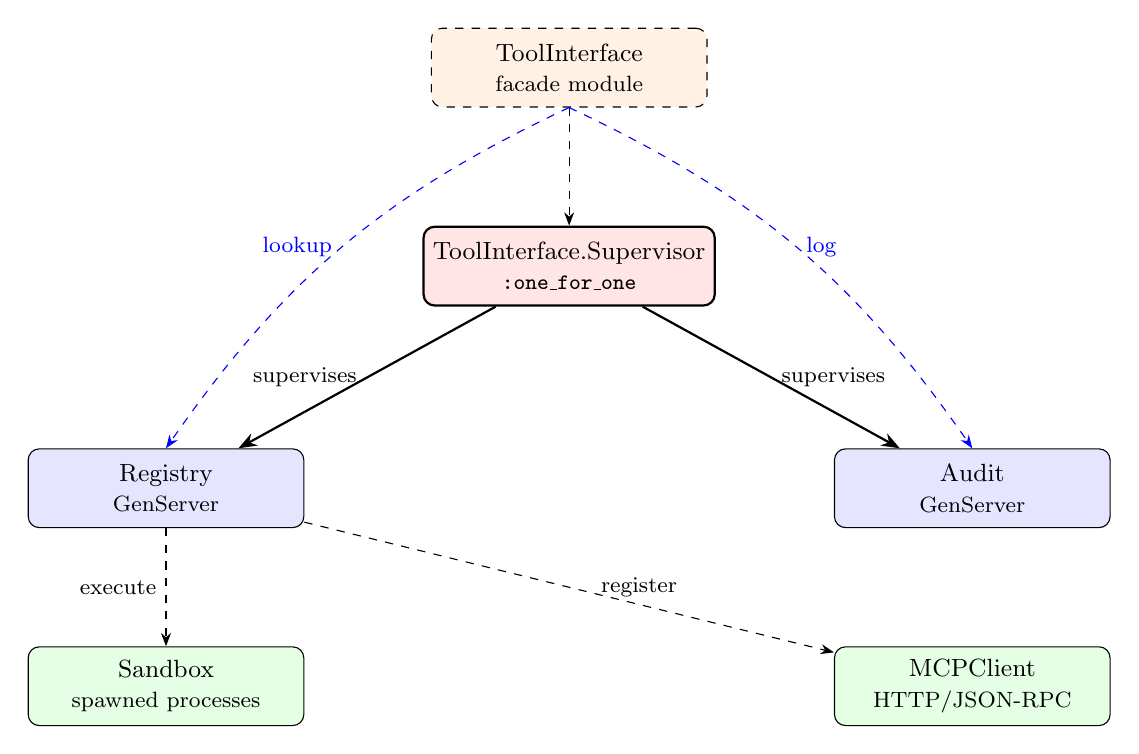
\begin{tikzpicture}[
  node distance=1.8cm,
  box/.style={draw, rounded corners, minimum width=3.5cm, minimum height=1cm, align=center, font=\small},
  supervisor/.style={box, fill=red!10, thick},
  genserver/.style={box, fill=blue!10},
  worker/.style={box, fill=green!10},
  facade/.style={box, fill=orange!10, dashed},
]
\node[supervisor] (app) {ToolInterface.Supervisor\\{\footnotesize\texttt{:one\_for\_one}}};
\node[genserver, below left=1.8cm and 1.5cm of app] (reg) {Registry\\{\footnotesize GenServer}};
\node[genserver, below right=1.8cm and 1.5cm of app] (audit) {Audit\\{\footnotesize GenServer}};
\node[worker, below=1.5cm of reg] (sandbox) {Sandbox\\{\footnotesize spawned processes}};
\node[worker, below=1.5cm of audit] (mcp) {MCPClient\\{\footnotesize HTTP/JSON-RPC}};
\node[facade, above=1.5cm of app] (facade) {ToolInterface\\{\footnotesize facade module}};

\draw[-{Stealth}, thick] (app) -- (reg) node[midway, left, font=\footnotesize] {supervises};
\draw[-{Stealth}, thick] (app) -- (audit) node[midway, right, font=\footnotesize] {supervises};
\draw[-{Stealth}, dashed] (facade) -- (app);
\draw[-{Stealth}, dashed, blue] (facade.south) to[bend right=15] node[midway, left, font=\footnotesize] {lookup} (reg.north);
\draw[-{Stealth}, dashed, blue] (facade.south) to[bend left=15] node[midway, right, font=\footnotesize] {log} (audit.north);
\draw[-{Stealth}, dashed] (reg) -- (sandbox) node[midway, left, font=\footnotesize] {execute};
\draw[-{Stealth}, dashed] (reg) -- (mcp) node[midway, right=8pt, font=\footnotesize] {register};
\end{tikzpicture}
\caption{OTP supervision tree. Solid arrows represent supervision relationships. Dashed arrows represent function calls and message passing. The facade module is not a process---it coordinates calls to the supervised GenServers.}
\label{fig:otp-tree}
\end{figure}


% ===== 8. AUDIT AND OBSERVABILITY =====
\section{Audit Logger}
\label{sec:audit}

\subsection{Design: Asynchronous, Non-Blocking Logging}

The audit logger records every tool invocation with full context. It is implemented as a GenServer that receives log entries asynchronously via \texttt{GenServer.cast/2}, ensuring that audit overhead does not impact tool invocation latency.

\begin{designprinciple}[Non-Blocking Audit]
\label{dp:audit}
Audit logging must not add latency to tool invocations. The audit logger receives entries via asynchronous casts (fire-and-forget). Entries are accumulated in memory and periodically flushed to persistent storage.
\end{designprinciple}

\subsection{Entry Structure}

Each audit entry captures the complete invocation context:

\begin{lstlisting}[language=elixir, caption={Audit entry structure.}, label={lst:audit-entry}]
defmodule ToolInterface.Audit do
  use GenServer
  require Logger

  @type entry :: %{
    id: String.t(),           # unique entry ID
    timestamp: DateTime.t(),   # UTC timestamp
    agent_id: String.t(),      # who invoked
    tool_id: String.t(),       # what was invoked
    input: map(),              # sanitized input
    output: any(),             # sanitized output
    duration_ms: non_neg_integer(),  # execution time
    status: :ok | :error       # outcome
  }
end
\end{lstlisting}

\subsection{Asynchronous Logging with Telemetry}

The \texttt{log\_invocation} function constructs an entry, emits a telemetry event, and casts to the GenServer:

\begin{lstlisting}[language=elixir, caption={Audit logging with telemetry integration.}, label={lst:audit-log}]
def log_invocation(agent_id, tool_id, input, output,
                   duration_ms, status) do
  entry = %{
    id: generate_entry_id(),
    timestamp: DateTime.utc_now(),
    agent_id: agent_id,
    tool_id: tool_id,
    input: sanitize_for_logging(input),
    output: sanitize_for_logging(output),
    duration_ms: duration_ms,
    status: status
  }

  # Emit telemetry event for external observability
  :telemetry.execute(
    [:tool_interface, :invocation],
    %{duration_ms: duration_ms},
    %{agent_id: agent_id, tool_id: tool_id, status: status}
  )

  GenServer.cast(__MODULE__, {:log, entry})
end
\end{lstlisting}

The \texttt{:telemetry.execute/3} call emits a structured event that can be consumed by Prometheus exporters, StatsD clients, or any other telemetry backend. This integrates with the broader Erlang/Elixir observability ecosystem without coupling the audit logger to a specific monitoring system.

\subsection{Sensitive Data Sanitization}

Before logging, input and output data are sanitized to prevent credential leakage:

\begin{lstlisting}[language=elixir, caption={Recursive sensitive data sanitization.}, label={lst:sanitize}]
defp sanitize_for_logging(data) when is_map(data) do
  sensitive_keys = ["password", "token", "secret",
                    "api_key", "authorization"]

  Map.new(data, fn
    {key, _value} when is_binary(key) ->
      if String.downcase(key) in sensitive_keys do
        {key, "[REDACTED]"}
      else
        {key, sanitize_for_logging(Map.get(data, key))}
      end
    {key, value} ->
      {key, sanitize_for_logging(value)}
  end)
end

defp sanitize_for_logging(data) when is_list(data) do
  Enum.map(data, &sanitize_for_logging/1)
end

defp sanitize_for_logging(data), do: data
\end{lstlisting}

The sanitizer recursively traverses maps and lists, replacing values at sensitive keys with \texttt{[REDACTED]}. This prevents Bearer tokens, API keys, and passwords from appearing in audit logs.

\subsection{Ring Buffer with Capacity Bounds}

The GenServer maintains entries in a bounded ring buffer:

\begin{lstlisting}[language=elixir, caption={Ring buffer entry storage with capacity bounds.}, label={lst:ring-buffer}]
defstruct entries: [],
          entry_count: 0,
          max_entries: 10_000,
          flush_interval_ms: 60_000

@impl true
def handle_cast({:log, entry}, state) do
  Logger.debug(
    "[Audit] #{entry.agent_id} -> #{entry.tool_id} " <>
    "[#{entry.status}] #{entry.duration_ms}ms"
  )

  entries =
    if state.entry_count >= state.max_entries do
      # Drop oldest entry when at capacity
      [entry | Enum.take(state.entries, state.max_entries - 1)]
    else
      [entry | state.entries]
    end

  new_count = min(state.entry_count + 1, state.max_entries)
  {:noreply, %{state | entries: entries, entry_count: new_count}}
end
\end{lstlisting}

When the buffer reaches capacity (default 10,000 entries), the oldest entry is dropped. This prevents unbounded memory growth in long-running systems. Periodic flushing to persistent storage ensures that entries survive process restarts.

\subsection{Periodic Flushing}

The audit GenServer schedules periodic flushes using \texttt{Process.send\_after}:

\begin{lstlisting}[language=elixir, caption={Periodic flush scheduling.}, label={lst:flush}]
@impl true
def init(opts) do
  max_entries = Keyword.get(opts, :max_entries, 10_000)
  flush_interval = Keyword.get(opts, :flush_interval_ms, 60_000)

  state = %__MODULE__{
    entries: [],
    entry_count: 0,
    max_entries: max_entries,
    flush_interval_ms: flush_interval
  }

  if flush_interval > 0 do
    Process.send_after(self(), :periodic_flush, flush_interval)
  end

  {:ok, state}
end

@impl true
def handle_info(:periodic_flush, state) do
  if state.entry_count > 0 do
    do_flush(state.entries)
  end
  Process.send_after(self(), :periodic_flush,
                     state.flush_interval_ms)
  {:noreply, state}
end
\end{lstlisting}

The flush mechanism uses \texttt{handle\_info} to process the self-sent \texttt{:periodic\_flush} message. In production, \texttt{do\_flush} would write to a database, object storage, or streaming pipeline (Kafka, CloudWatch, etc.). The reference implementation retains entries in memory only.

\subsection{Query and Statistics}

The audit logger supports querying entries and computing aggregate statistics:

\begin{lstlisting}[language=elixir, caption={Audit statistics computation.}, label={lst:stats}]
defp compute_stats(entries) do
  total = length(entries)
  ok_count = Enum.count(entries, &(&1.status == :ok))
  error_count = total - ok_count
  total_duration = Enum.reduce(entries, 0,
                               &(&1.duration_ms + &2))
  avg_duration = if total > 0,
                    do: total_duration / total,
                    else: 0.0

  %{
    total: total,
    ok: ok_count,
    error: error_count,
    avg_duration_ms: Float.round(avg_duration, 2),
    tools_used: entries
                |> Enum.map(& &1.tool_id)
                |> Enum.uniq()
                |> length(),
    agents_active: entries
                   |> Enum.map(& &1.agent_id)
                   |> Enum.uniq()
                   |> length()
  }
end
\end{lstlisting}

The pipeline operator makes the data flow readable: take the entries, extract tool IDs, remove duplicates, count. This computes six aggregate metrics: total invocations, success count, error count, average duration, unique tools used, and active agents.


% ===== 9. PRODUCTION MAPPING =====
\section{Production Validation: Mapping to Agent-Hero}
\label{sec:production}

The reference implementation's design maps directly to the \agenthero{} production platform. This section traces the correspondence between the Elixir reference implementation and the deployed TypeScript/Next.js system.

\subsection{Three-Tier Model Correspondence}

\begin{center}
\begin{tabularx}{\textwidth}{lXX}
\toprule
\textbf{Tier} & \textbf{Elixir Reference} & \textbf{Agent-Hero Production} \\
\midrule
Builtin & Static tool specs in \texttt{Registry.init/1} & Vercel AI SDK \texttt{tool()} definitions with Zod schemas \\
Sandbox & \texttt{Sandbox.execute/3} spawning isolated BEAM processes & E2B Code Interpreter with 10-minute ephemeral sandboxes \\
MCP & \texttt{MCPClient.discover\_and\_register/3} via Finch HTTP & \texttt{StreamableHTTPClientTransport} from \texttt{@modelcontextprotocol/sdk} \\
\bottomrule
\end{tabularx}
\end{center}

\subsection{Capability Token Correspondence}

In the Elixir implementation, capability tokens are HMAC-signed structs with TTL, rate limiting, and permission scoping. In \agenthero{}, the same security model is implemented through per-agent tool permissions stored in the database:

\begin{lstlisting}[language=typescript, caption={Agent-Hero tool permission model (simplified).}, label={lst:ah-permissions}]
// Agent-Hero: per-agent tool permissions
const frozenTools = Object.freeze(
  resolveToolsForAgent(agent, contract)
);

// Tool set is immutable during execution
async function executeAgent(agent, task) {
  const tools = frozenTools;
  return await runAgentLoop(agent, task, tools);
}
\end{lstlisting}

The \texttt{Object.freeze()} in TypeScript corresponds to \texttt{Registry.freeze()} in Elixir. Both ensure that the tool set is immutable during agent execution.

\subsection{Sandbox Correspondence}

The Elixir sandbox uses BEAM process isolation with \texttt{spawn\_monitor} and hard timeouts. The \agenthero{} platform uses E2B sandboxes with the same 10-minute timeout:

\begin{lstlisting}[language=typescript, caption={E2B sandbox execution in Agent-Hero.}, label={lst:e2b}]
import { Sandbox } from '@e2b/code-interpreter';

async function executeSandboxed(code: string, language: string) {
  const sandbox = await Sandbox.create({
    timeoutMs: 10 * 60 * 1000,  // 10 minutes
  });
  try {
    const result = await sandbox.runCode(code, { language });
    return {
      stdout: result.logs.stdout,
      stderr: result.logs.stderr,
      exitCode: result.exitCode,
    };
  } finally {
    await sandbox.close();  // ephemeral: always clean up
  }
}
\end{lstlisting}

The correspondence is direct: \texttt{spawn\_monitor} maps to \texttt{Sandbox.create}, the \texttt{after timeout} clause maps to \texttt{timeoutMs}, and \texttt{Process.exit(pid, :kill)} maps to the implicit sandbox termination.

\subsection{MCP Correspondence}

The Elixir MCP client's \texttt{discover\_all} with \texttt{Task.async\_stream} maps to \agenthero{}'s parallel server connection:

\begin{lstlisting}[language=typescript, caption={Parallel MCP discovery in Agent-Hero.}, label={lst:ah-mcp}]
const connections = await Promise.allSettled(
  mcpServers.map(async (server) => {
    const transport = new StreamableHTTPClientTransport(
      new URL(server.url),
      { headers: { Authorization: `Bearer ${server.token}` } }
    );
    const client = new Client({
      name: "agent-hero", version: "1.0"
    });
    await client.connect(transport);
    const { tools } = await client.listTools();
    return tools.map(t => ({
      name: `${server.name}__${t.name}`,
      description: t.description,
      schema: t.inputSchema,
    }));
  })
);
\end{lstlisting}

\texttt{Task.async\_stream} with \texttt{on\_timeout: :kill\_task} provides the same semantics as \texttt{Promise.allSettled}: each server is handled independently, failures are isolated, and the system proceeds with whatever tools were successfully discovered.

\subsection{Audit Correspondence}

The Elixir audit logger's telemetry integration maps to \agenthero{}'s credit-based billing system, where each tool invocation consumes credits proportional to execution time and API costs. The audit entry's \texttt{duration\_ms} field directly feeds the billing computation.


% ===== 10. DESIGN ANALYSIS =====
\section{Design Analysis and Comparisons}
\label{sec:analysis}

\subsection{Comparison to Classical Operating System Patterns}

\begin{center}
\begin{tabularx}{\textwidth}{lXX}
\toprule
\textbf{Classical OS Concept} & \textbf{AI OS Equivalent} & \textbf{Elixir Implementation} \\
\midrule
File descriptor & Capability token & \texttt{Capability.t()} struct \\
Device driver & Tool implementation & \texttt{tool\_spec.execute} function \\
System call & Tool invocation & \texttt{ToolInterface.invoke/4} \\
\texttt{/dev} directory & Tool registry & \texttt{Registry} GenServer \\
Major/minor numbers & Tier + tool ID & \texttt{:builtin | :sandbox | :mcp} + string \\
\texttt{ioctl} parameters & Tool input schema & JSON Schema map \\
Kernel ring 0 & Builtin tier & Direct function execution \\
User-space ring 3 & Sandbox tier & Spawned BEAM process \\
Network driver & MCP tier & HTTP/JSON-RPC closure \\
\texttt{open()} permission & Capability authorization & \texttt{Capability.authorize/2} \\
\texttt{close()} cleanup & Token revocation & \texttt{Capability.revoke/1} \\
\bottomrule
\end{tabularx}
\end{center}

The key difference is that the AI OS must handle \emph{dynamic} tool discovery (through MCP) whereas Unix device discovery is largely static. The freeze mechanism bridges this gap: tools are discovered dynamically but frozen at execution time, providing the stability guarantees of static configuration.

\subsection{Comparison to Plan 9}

Plan~9's ``everything is a file'' philosophy~\citep{pike1995plan9} suggests that the AI OS should present all tools through a uniform interface. MCP achieves this: every tool, regardless of implementation, is invoked through the same JSON-RPC protocol with the same schema-based input/output contract.

Plan~9 goes further with \emph{per-process name spaces}: each process sees a different file system tree. The AI OS analogue is per-agent capability scoping: each agent's tokens define a different view of the tool registry, restricted to the tools the agent is authorized to use.

\subsection{Comparison to Capsicum and seL4}

Capsicum~\citep{watson2010capsicum} and seL4~\citep{klein2009sel4} provide the closest security analogues:

\begin{itemize}[leftmargin=2em]
\item \textbf{Capsicum's capability mode} is directly analogous to registry freezing. Once an execution begins, no new capabilities can be acquired.
\item \textbf{seL4's per-syscall capabilities} are analogous to per-invocation token authorization. Every tool call requires a valid capability token.
\item \textbf{seL4's formal verification} is a goal for future work. The current system relies on Elixir's type specifications and runtime validation rather than machine-checked proofs.
\end{itemize}

\subsection{Functional Composition Properties}

The tool interface design inherits several useful properties from functional programming:

\begin{proposition}[Composition Associativity]
For any three tools $f$, $g$, $h$ whose types align (the output type of $f$ matches the input type of $g$, and the output type of $g$ matches the input type of $h$), the composition is associative:
\[
  x \pipe f \pipe g \pipe h = x \pipe f \pipe (g \pipe h) = x \pipe (f \pipe g) \pipe h
\]
\end{proposition}

This follows directly from the fact that tool execution is function application, and function composition is associative. In practical terms, it means that tool pipelines can be freely refactored---extracting a sub-pipeline into a named composition, or inlining a named composition into a larger pipeline---without changing behavior.

\begin{proposition}[Type-Safe Composition]
If tool $f$ produces output conforming to schema $\sigma_B$ and tool $g$ accepts input conforming to schema $\sigma_B$, then the composition $f \pipe g$ preserves type correctness: valid input to $f$ produces valid input to $g$.
\end{proposition}

This is enforced at runtime through the validation pipeline: each tool's \texttt{validate} function checks its input before execution. Schema-level composition checking (verifying that output schemas match input schemas before execution begins) is a natural extension for future work.

\subsection{Security Properties}

\begin{proposition}[Sandbox Isolation]
If two agents $a$ and $b$ have disjoint capability sets (no shared tokens), and all sandbox executions run in separate BEAM processes, then no direct information flow exists between $a$'s tool executions and $b$'s tool executions.
\end{proposition}

This follows from BEAM process isolation: each process has its own heap, and inter-process communication requires explicit message passing. A sandbox process for agent $a$ cannot read the memory of a sandbox process for agent $b$, and the capability system prevents $a$ from invoking tools authorized only for $b$.

\begin{remark}[Limitations]
This isolation guarantee does not address timing side channels (observable differences in execution duration), resource-usage side channels (observable memory or CPU consumption), or prompt injection attacks (external content containing adversarial instructions). These require additional countermeasures beyond the tool interface layer.
\end{remark}

\subsection{Scalability Properties}

The BEAM virtual machine provides strong scalability properties for the tool interface:

\begin{itemize}[leftmargin=2em]
\item \textbf{Concurrent invocations}: The BEAM scheduler handles millions of lightweight processes, enabling massive concurrent tool execution.
\item \textbf{Fault isolation}: A crashing tool affects only its own process. The registry, audit logger, and other tool executions are unaffected.
\item \textbf{Back-pressure}: The GenServer message queue provides natural back-pressure. If the registry is overwhelmed with lookup requests, callers block on \texttt{GenServer.call}, creating upstream pressure.
\item \textbf{Distribution}: OTP distribution allows the registry to span multiple nodes. Capability tokens are validated locally (HMAC verification requires only the signing key, not a database lookup).
\end{itemize}


% ===== 11. CASE STUDIES =====
\section{Case Studies}
\label{sec:case-studies}

\subsection{Web Scraping Pipeline}

Consider an agent tasked with extracting structured data from the web. The pipeline composes three builtin tools:

\begin{lstlisting}[language=elixir, caption={Web scraping pipeline composing three tools.}, label={lst:web-pipeline}]
# Grant capabilities for each tool in the pipeline
{:ok, search_cap} = ToolInterface.grant_capability(
  "agent-1", "web-search", permissions: [:invoke])
{:ok, scrape_cap} = ToolInterface.grant_capability(
  "agent-1", "web-scrape", permissions: [:invoke])
{:ok, transform_cap} = ToolInterface.grant_capability(
  "agent-1", "text-transform", permissions: [:invoke])

# Step 1: Search
{:ok, urls} = ToolInterface.invoke(
  "agent-1", "web-search",
  %{"query" => "elixir otp patterns"}, search_cap)

# Step 2: Scrape (URL safety validated automatically)
{:ok, html} = ToolInterface.invoke(
  "agent-1", "web-scrape",
  %{"url" => hd(urls.results)}, scrape_cap)

# Step 3: Transform
{:ok, structured} = ToolInterface.invoke(
  "agent-1", "text-transform",
  %{"text" => html.content, "operation" => "extract"},
  transform_cap)
\end{lstlisting}

Each invocation goes through the full pipeline: capability authorization, registry lookup, input validation (including URL safety for the scrape step), execution, and audit logging. The URL safety validator blocks any attempt to scrape \texttt{localhost} or private IP ranges, preventing SSRF attacks.

\subsection{Sandboxed Code Execution}

Code execution tools run in isolated BEAM processes:

\begin{lstlisting}[language=elixir, caption={Sandboxed code execution with timeout.}, label={lst:code-exec}]
{:ok, exec_cap} = ToolInterface.grant_capability(
  "agent-2", "code-exec",
  permissions: [:invoke], rate_limit: 10)

# Executes in a separate BEAM process with 10-min timeout
{:ok, result} = ToolInterface.invoke(
  "agent-2", "code-exec",
  %{"code" => "Enum.sum(1..100)", "language" => "elixir"},
  exec_cap)

# If execution exceeds timeout:
# {:error, :timeout}

# If code raises an exception:
# {:error, {:execution_failed, "ArithmeticError: ..."}}

# If sandbox process crashes:
# {:error, {:sandbox_crashed, :normal}}
\end{lstlisting}

The rate limit of 10 invocations per minute prevents an agent from spawning too many sandbox processes. Each error case produces a distinct tagged tuple, enabling precise error handling and reporting.

\subsection{Multi-MCP Server Discovery}

At execution startup, the platform discovers tools from multiple MCP servers:

\begin{lstlisting}[language=elixir, caption={Multi-server MCP discovery and freeze.}, label={lst:multi-mcp}]
servers = [
  %{name: "github", url: "https://mcp.github.com",
    token: "ghp_..."},
  %{name: "slack", url: "https://mcp.slack.com",
    token: "xoxb-..."},
  %{name: "jira", url: "https://mcp.jira.com",
    token: "jira_..."}
]

# Discover in parallel - failures are isolated
results = ToolInterface.MCPClient.discover_all(servers,
  max_concurrency: 10, timeout: 30_000)

# results might be:
# [{:ok, "github"}, {:ok, "slack"},
#  {:error, "jira", :connection_refused}]

# Freeze the registry - no more tools can be added
ToolInterface.freeze()

# Agent can now use: github__create_issue, slack__send_message
# but NOT any jira tools (discovery failed)
# and cannot discover new servers (registry frozen)
\end{lstlisting}

The parallel discovery ensures that a slow Jira server does not delay GitHub and Slack tool availability. After freezing, the tool set is immutable for the duration of the agent execution.

\begin{figure}[ht]
\centering
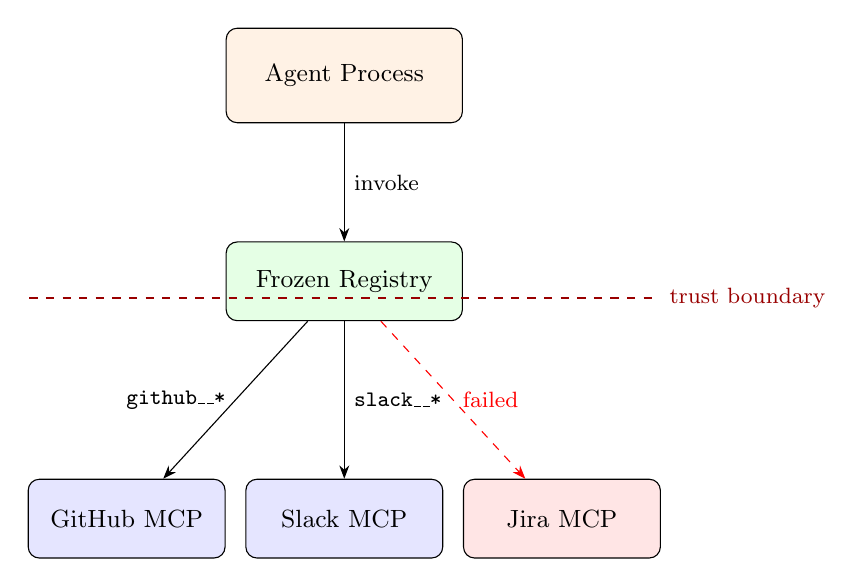
\begin{tikzpicture}[
  node distance=2cm,
  server/.style={draw, rounded corners, minimum width=2.5cm, minimum height=1cm, fill=blue!10, font=\small},
  agent/.style={draw, rounded corners, minimum width=3cm, minimum height=1.2cm, fill=orange!10, font=\small},
  registry/.style={draw, rounded corners, minimum width=3cm, minimum height=1cm, fill=green!10, font=\small},
]
\node[agent] (agent) {Agent Process};
\node[registry, below=1.5cm of agent] (reg) {Frozen Registry};
\node[server, below left=2cm and 0cm of reg] (s1) {GitHub MCP};
\node[server, below=2cm of reg] (s2) {Slack MCP};
\node[server, below right=2cm and 0cm of reg, fill=red!10] (s3) {Jira MCP};

\draw[-{Stealth}] (agent) -- (reg) node[midway, right, font=\footnotesize] {invoke};
\draw[-{Stealth}] (reg) -- (s1) node[midway, left, font=\footnotesize] {\texttt{github\_\_*}};
\draw[-{Stealth}] (reg) -- (s2) node[midway, right, font=\footnotesize] {\texttt{slack\_\_*}};
\draw[-{Stealth}, dashed, red] (reg) -- (s3) node[midway, right, font=\footnotesize\color{red}] {failed};

\draw[dashed, red!60!black, thick] ([xshift=-4cm, yshift=0.3cm]reg.south) -- ([xshift=4cm, yshift=0.3cm]reg.south) node[right, font=\footnotesize\color{red!60!black}] {trust boundary};
\end{tikzpicture}
\caption{Multi-MCP server orchestration. The Jira connection failed, but GitHub and Slack tools are available. The registry is frozen after discovery.}
\label{fig:multi-mcp}
\end{figure}


% ===== 12. SECURITY LIMITATIONS =====
\section{Security Limitations and Future Directions}
\label{sec:limitations}

\subsection{Known Limitations}

The tool interface design has several limitations:

\begin{enumerate}[leftmargin=2em]
\item \textbf{Side channels}: Sandbox isolation prevents direct data flow between agents but does not address timing side channels or resource-usage side channels.

\item \textbf{Tool implementation trust}: We assume tool implementations are correct with respect to their schemas. A malicious tool implementation could violate type contracts.

\item \textbf{MCP server trust}: MCP-discovered tools rely on the security of external servers. A compromised server could provide tools with misleading descriptions or malicious implementations.

\item \textbf{Prompt injection}: Tools that process external content (e.g., \texttt{web-scrape}) may return data containing prompt injection attacks. The type system validates structure but not semantic content.

\item \textbf{Signing key management}: The current implementation uses a hardcoded signing key. Production deployment requires integration with a secrets manager (AWS KMS, HashiCorp Vault, etc.).

\item \textbf{Capability delegation}: The current model does not support agent-to-agent capability delegation. An agent cannot grant a subset of its capabilities to a sub-agent.
\end{enumerate}

\subsection{Future Directions}

\begin{enumerate}[leftmargin=2em]
\item \textbf{Capability delegation}: Allowing agents to delegate subsets of their capabilities to sub-agents, with formal guarantees that delegated capabilities cannot exceed the delegator's authority.

\item \textbf{Schema-level composition checking}: Verifying at registration time that composed tool pipelines have compatible input/output schemas, catching type mismatches before execution.

\item \textbf{Formal verification}: Machine-checking the security properties using property-based testing (StreamData in Elixir) or formal verification tools (Lean 4, TLA+).

\item \textbf{Differential privacy}: Extending the audit system with differential privacy guarantees on aggregated tool usage statistics.

\item \textbf{WebAssembly sandboxing}: Adding a WASI-based sandbox tier for tools that require stronger isolation than BEAM processes provide (e.g., tools executing untrusted native code).

\item \textbf{Distributed registry}: Extending the registry to span multiple BEAM nodes using distributed Erlang, with capability tokens validated locally and tool state replicated via CRDTs.
\end{enumerate}


% ===== 13. RELATED WORK =====
\section{Related Work}
\label{sec:related}

\subsection{Tool Use in Language Models}

The emergence of tool-augmented language models~\citep{schiller2024toolformer} has created a need for structured tool interfaces. OpenAI's function calling~\citep{openai2024function} provides JSON Schema-based tool definitions, and the Vercel AI SDK~\citep{vercel2024aisdk} extends this with type-safe tool definitions using Zod schemas. The Model Context Protocol~\citep{mcp2024spec} standardizes tool discovery and invocation across providers.

Our contribution is orthogonal to these interfaces: we focus on the operating system layer that manages, secures, and audits tool access, regardless of which tool invocation protocol is used at the application layer.

\subsection{Capability-Based Security}

The capability security literature~\citep{dennis1966capabilities,levy1984capability,miller2003capability} provides the theoretical foundation for our token model. Capsicum~\citep{watson2010capsicum} and seL4~\citep{klein2009sel4} demonstrate that capabilities can be both practical and formally verifiable. Macaroons~\citep{birgisson2014macaroons} extend capabilities with contextual caveats, a direction we may pursue for conditional tool access.

\subsection{Actor Model and BEAM}

The BEAM virtual machine realizes the actor model~\citep{hewitt1973actors} with added supervision and hot-code loading~\citep{armstrong2003erlang}. The tool interface's use of process isolation for sandboxing is a natural application of BEAM's architectural properties. Juric~\citep{juric2019elixir} and Thomas~\citep{thomas2018elixir} provide comprehensive treatments of Elixir/OTP patterns that inform our GenServer and supervision designs.

\subsection{Operating System Abstractions}

Tanenbaum and Bos~\citep{tanenbaum2014modern} survey modern OS design. Love~\citep{love2010linux} details the Linux kernel's device driver model. Pike et al.~\citep{pike1995plan9} describe Plan~9's uniform resource abstraction. Ritchie and Thompson~\citep{ritchie1978unix} established the foundational Unix abstractions. Our tool interface layer draws on all of these traditions, adapting them to the AI agent context.


% ===== 14. CONCLUSION =====
\section{Conclusion}
\label{sec:conclusion}

We have presented the design and implementation of a tool interface layer for an AI Operating System. The key contributions are:

\begin{enumerate}[leftmargin=2em]
\item A \textbf{three-tier tool registry} (Builtin, Sandbox, MCP) implemented as an Elixir GenServer with freeze semantics that lock the tool set at execution time, preventing privilege escalation.

\item A \textbf{capability token system} using HMAC-SHA256 signed tokens with TTL, rate limiting, and permission scoping, providing decentralized authorization without central bottlenecks.

\item A \textbf{process-isolated sandbox executor} using BEAM \texttt{spawn\_monitor} with hard timeouts, providing the same isolation guarantees as E2B ephemeral environments at the language-runtime level.

\item An \textbf{MCP protocol client} with session management, parallel multi-server discovery, and closure-based remote executors that make network boundaries transparent.

\item An \textbf{asynchronous audit logger} with telemetry integration, sensitive data sanitization, and bounded ring-buffer storage.

\item A \textbf{facade module} that composes these components into a single invocation pipeline: authorize, lookup, validate, execute, audit.
\end{enumerate}

The tool interface layer is the bridge between intelligence and action. Just as Unix's device driver model enabled a rich ecosystem of applications by abstracting hardware complexity, the AI OS tool layer enables a rich ecosystem of agents by abstracting the complexity of external system interaction. The functional design ensures that tools compose cleanly, capabilities are enforced at every invocation, execution is isolated by trust level, and every action is auditable.

The Elixir/OTP reference implementation demonstrates that the BEAM virtual machine---with its per-process heap isolation, preemptive scheduling, and supervision trees---is a natural fit for implementing operating system abstractions. The approximately 700 lines of Elixir that constitute the reference implementation provide the same security and reliability guarantees that classical operating systems achieve through hardware protection rings, but with the development velocity and composability of a high-level functional language.

In Part~III of this series, we turn to the memory and persistence layer---the mechanism by which agents maintain state across interactions, leveraging Elixir's ETS tables, persistent term storage, and distributed state management.


% ===== REFERENCES =====
\newpage
\bibliographystyle{plainnat}

\begin{thebibliography}{35}

\bibitem[Armstrong(2003)]{armstrong2003erlang}
Armstrong, J. (2003).
\newblock \emph{Making Reliable Distributed Systems in the Presence of Software Errors}.
\newblock PhD thesis, Royal Institute of Technology, Stockholm.

\bibitem[Birgisson et~al.(2014)]{birgisson2014macaroons}
Birgisson, A., Politz, J.~G., Erlingsson, \'{U}., Taly, A., Vrable, M., and Lentczner, M. (2014).
\newblock Macaroons: Cookies with contextual caveats for decentralized authorization in the cloud.
\newblock In \emph{NDSS 2014}.

\bibitem[Brown et~al.(2020)]{brown2020gpt3}
Brown, T.~B., Mann, B., Ryder, N., et~al. (2020).
\newblock Language models are few-shot learners.
\newblock In \emph{NeurIPS 2020}.

\bibitem[Cesarini \& Thompson(2009)]{cesarini2009erlang}
Cesarini, F. and Thompson, S. (2009).
\newblock \emph{Erlang Programming}.
\newblock O'Reilly Media.

\bibitem[Dennis \& Van~Horn(1966)]{dennis1966capabilities}
Dennis, J.~B. and Van~Horn, E.~C. (1966).
\newblock Programming semantics for multiprogrammed computations.
\newblock \emph{Communications of the ACM}, 9(3):143--155.

\bibitem[E2B(2024)]{e2b2024docs}
E2B (2024).
\newblock E2B Code Interpreter documentation.
\newblock \url{https://e2b.dev/docs}.

\bibitem[Fong \& Spivak(2019)]{fong2019seven}
Fong, B. and Spivak, D.~I. (2019).
\newblock \emph{An Invitation to Applied Category Theory: Seven Sketches in Compositionality}.
\newblock Cambridge University Press.

\bibitem[Hardy(1988)]{hardy1988keykos}
Hardy, N. (1988).
\newblock The KeyKOS architecture.
\newblock \emph{ACM SIGOPS Operating Systems Review}, 19(4):8--25.

\bibitem[Hewitt et~al.(1973)]{hewitt1973actors}
Hewitt, C., Bishop, P., and Steiger, R. (1973).
\newblock A universal modular ACTOR formalism for artificial intelligence.
\newblock In \emph{IJCAI 1973}, pages 235--245.

\bibitem[Juric(2019)]{juric2019elixir}
Juric, S. (2019).
\newblock \emph{Elixir in Action}.
\newblock Manning Publications, 2nd edition.

\bibitem[Klein et~al.(2009)]{klein2009sel4}
Klein, G., Elphinstone, K., Heiser, G., et~al. (2009).
\newblock seL4: Formal verification of an OS kernel.
\newblock In \emph{SOSP 2009}, pages 207--220.

\bibitem[Levy(1984)]{levy1984capability}
Levy, H.~M. (1984).
\newblock \emph{Capability-Based Computer Systems}.
\newblock Digital Press.

\bibitem[Long(2026a)]{longyoneda2026kernel}
Long, M. (2026a).
\newblock The AI Operating System, Part~I: Kernel architecture---process model, scheduling, and categorical foundations.
\newblock \emph{GrokRxiv preprint}, 2026.03.

\bibitem[Love(2010)]{love2010linux}
Love, R. (2010).
\newblock \emph{Linux Kernel Development}.
\newblock Addison-Wesley, 3rd edition.

\bibitem[Miller et~al.(2003)]{miller2003capability}
Miller, M.~S., Yee, K.-P., and Shapiro, J. (2003).
\newblock Capability myths demolished.
\newblock Technical report, HP Laboratories.

\bibitem[MCP~Specification(2024)]{mcp2024spec}
Model Context Protocol Working Group (2024).
\newblock Model Context Protocol specification, version 1.0.
\newblock \url{https://modelcontextprotocol.io/specification}.

\bibitem[Moggi(1991)]{moggi1991notions}
Moggi, E. (1991).
\newblock Notions of computation and monads.
\newblock \emph{Information and Computation}, 93(1):55--92.

\bibitem[OpenAI(2024)]{openai2024function}
OpenAI (2024).
\newblock Function calling --- OpenAI API documentation.
\newblock \url{https://platform.openai.com/docs/guides/function-calling}.

\bibitem[Pike et~al.(1995)]{pike1995plan9}
Pike, R., Presotto, D., Dorward, S., Flandrena, B., Thompson, K., Trickey, H., and Winterbottom, P. (1995).
\newblock Plan~9 from Bell Labs.
\newblock \emph{Computing Systems}, 8(3):221--254.

\bibitem[Ritchie \& Thompson(1978)]{ritchie1978unix}
Ritchie, D.~M. and Thompson, K. (1978).
\newblock The UNIX time-sharing system.
\newblock \emph{Bell System Technical Journal}, 57(6):1905--1929.

\bibitem[Schick et~al.(2024)]{schiller2024toolformer}
Schick, T., Dwivedi-Yu, J., Dess\`{\i}, R., et~al. (2024).
\newblock Toolformer: Language models can teach themselves to use tools.
\newblock In \emph{NeurIPS 2023}.

\bibitem[Shapiro \& Miller(2023)]{shapiro2023ocap}
Shapiro, J.~S. and Miller, M.~S. (2023).
\newblock Object-capability security: A retrospective.
\newblock \emph{IEEE Security \& Privacy}, 21(2):63--71.

\bibitem[Tanenbaum \& Bos(2014)]{tanenbaum2014modern}
Tanenbaum, A.~S. and Bos, H. (2014).
\newblock \emph{Modern Operating Systems}.
\newblock Pearson, 4th edition.

\bibitem[Thomas(2018)]{thomas2018elixir}
Thomas, D. (2018).
\newblock \emph{Programming Elixir 1.6}.
\newblock Pragmatic Bookshelf.

\bibitem[Vercel(2024)]{vercel2024aisdk}
Vercel (2024).
\newblock Vercel AI SDK documentation, v6.
\newblock \url{https://sdk.vercel.ai/docs}.

\bibitem[Wadler(1995)]{wadler1995monads}
Wadler, P. (1995).
\newblock Monads for functional programming.
\newblock In \emph{Advanced Functional Programming}, LNCS 925, pages 24--52. Springer.

\bibitem[WASI~Working~Group(2023)]{wasi2023spec}
WASI Working Group (2023).
\newblock WebAssembly System Interface specification.
\newblock \url{https://wasi.dev}.

\bibitem[Watson et~al.(2010)]{watson2010capsicum}
Watson, R.~N.~M., Anderson, J., Laurie, B., and Kennaway, K. (2010).
\newblock Capsicum: Practical capabilities for UNIX.
\newblock In \emph{USENIX Security 2010}, pages 29--46.

\end{thebibliography}

\end{document}
